\chapter{液体火箭发动机}
\thispagestyle{empty}
\section{液体火箭发动机组成及分类}
\subsection{液体火箭发动机的特点}
\vspace*{-1.5em}
\defination[液体火箭发动机 (Liquid Rockct Engine —  LRE)]
{
	\dy[液体火箭发动机]{YTHJFDJ}\quad 液体推进剂火箭发动机的简称,是使用液态化学物质作为能源和工质的化学火箭发动机,属于喷气发动机。
}
\noindent 其特点为:\vspace*{-0.8em}
\begin{itemize}
	\item 性能高,推力大\vspace*{-0.8em}
	\item 工作时间长短可以调整,可以多次启动、关机和重复使用\vspace*{-0.8em}
	\item 方便地调节推力大小和方向\vspace*{-0.8em}
	\item 结构质量小,推进剂消耗量大
\end{itemize}

\subsection{液体火箭发动机的基本组成}
基本组成有:\underline{推力室组件}、\underline{推进剂供应与控制系统}、\underline{阀门与调节器}、\underline{发动机总装元件}等。
\vspace*{0.5em}

\sssection[推力室组件]
\vspace*{-1em}
\begin{enumerate}[\hspace*{1.5em} (1) ]
	\item \textbf{功能} \hspace*{1em} 发动机燃烧和产生推力的组件。\vspace*{-0.8em}
	\item \textbf{构成} \hspace*{1em} 喷注器、燃烧室、喷管和点火装置(对非自然推进剂),如图\ref{推力室}所示。
	\begin{figure}[!htb]
		\centering
		\begin{minipage}{0.4\linewidth}
			\centering
			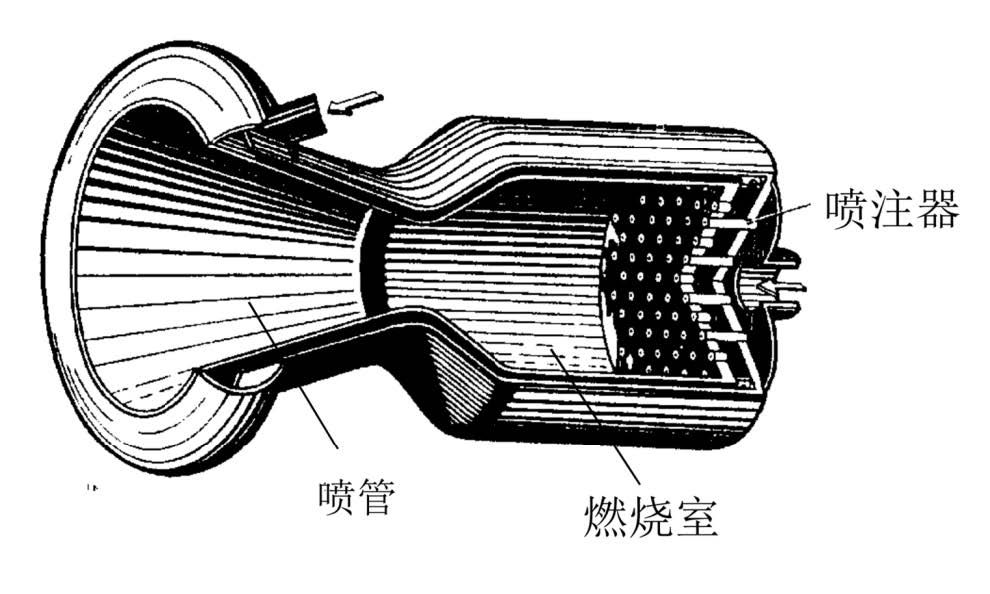
\includegraphics[width=\linewidth]{pic/推力室.jpg}
			\vspace*{-3em}
			\caption{推力室总体示意图}
			\label{推力室}
		\end{minipage}
		\begin{minipage}{0.45\linewidth}
			\centering
			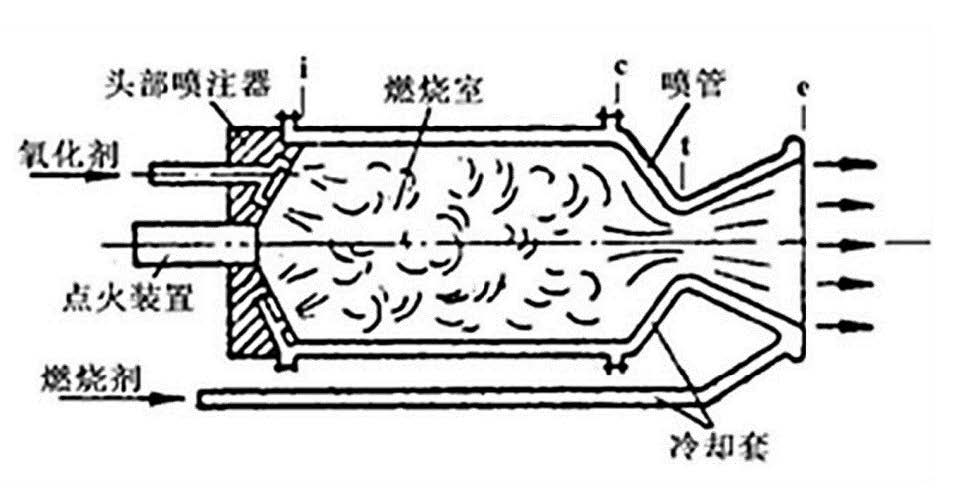
\includegraphics[width=\linewidth]{pic/推力室2.jpg}
			\vspace*{-2.8em}
			\caption{推力室内部示意图}
			\label{推力室2}
		\end{minipage}
	\end{figure}
	\vspace*{-1em}
	\item \textbf{工作过程} \hspace*{1em} 液体推进剂以\blue[规定的流量]和\blue[混合比]通过喷注器\blue[喷入燃烧室],在燃烧室内经过\blue[雾化、蒸发、混合和燃烧]等过程,产生的\blue[高温、高压燃气]在喷管内膨胀加速,以\blue[超声速]排出,从而产生推力。
	\item \textbf{特点} \hspace*{1em} \red[高温、高压环境],$3000\, \sim \, 4000 \degree\text{C}$,可以达到20$\,$MPa;\\
	\hspace*{3.5em}\red[化学反应速度很快,燃烧前准备过程决定燃烧速度]
\end{enumerate}

\sssection[推进剂供应系统]


\section{液体推进剂}
\subsection{液体推进剂分类及性能要求}
液体推进剂是翼液体状态进入推力室的推进剂,包括氧化剂和燃料以及单组元推进剂;可以是单质、化合物或混合物,是液体火箭发动机的能源和工质源,其质量占运载火箭起飞质量的70\% $\, \sim \,$90\%,直接影响着运载火箭和发动机的性能及制造费用。
\vspace*{0.5em}

\sssection[液体推进剂的分类]

\noindent \textbf{\underline{按进入推力室的基本组元数目分类}}
\vspace*{-0.5em}
\begin{enumerate}[\hspace*{1.5em} (1)  ]
	\item 单组元\\
	通过自身分解或燃烧能迅速产生高温高压的气体。\vspace*{-0.8em}
	\begin{enumerate}
		\item 在分子中同时含有可燃元素和燃烧所必需的氧的化合物,如:\underline{硝基甲烷、硝酸甲酯、过氧化氢} \vspace*{-0.5em}
		\item 在常压下互不产生化学反应的安定混合物,如:\underline{过氧化氢—甲醇}\vspace*{-0.5em}
		\item 在分解时能放出大量热量和气态产物的吸热化合物,如\underline{无水肼、甲基肼}\vspace*{-0.5em}
	\end{enumerate}
	单组元的特点:绝大多数单组元推进系统\blue[结构简单]、\blue[使用方便]、\blue[性能比较低]等\\
	单组元的应用:火箭发动机系统中的辅助能源,如涡轮泵燃气发生器、姿轨控制流
	
	\item 双组元\\
	由液体\red[燃烧剂]和\red[氧化剂]两种组员组成,工作时它们被分别从各自的贮箱和输送管路送入推力室。\vspace*{-0.8em}
	\begin{enumerate}
		\item 氧化剂:氧化力强的物质,如\underline{液氧、液氟、硝酸}等\vspace*{-0.5em}
		\item 燃烧剂(燃料):含氢量大、燃烧热值比较高的物质,如\underline{液氢、肼类、碳氢化合物}等\vspace*{-0.5em}
	\end{enumerate}
	双组元的特点:来源广泛、释放的能量较高\\
	双组元应用:液体火箭发动机绝大多数采用双组元推进剂
	
	\item 多组元
	由多于两组元组成的推进剂,常常指\dy[三组元]{SZY}。\vspace*{-0.8em}
	\begin{enumerate}
		\item 多于三组元的液体推进剂,理论上\red[能量不会进一步的增加]。\vspace*{-0.5em}
		\item 三组元足以能方便地把任何需要的化学元素组合起来。\vspace*{-0.5em}
	\end{enumerate}
	
	\item 三组元\vspace*{-0.8em}
	\begin{enumerate}
		\item 把轻金属(如锂、铍或铍的氢化物)同液氟、液氧或臭氧燃烧产生的高温与能够降低燃烧产物平均分子量的氢结合起来,提高比冲;\vspace*{-0.5em}
		\item 液氢、液氧和煤油 :在下面级工作时,常以氧为氧化剂、煤油为燃料并加入少量液氢燃料;\vspace*{-0.5em}
		\item 双燃料双膨胀:高压的内燃室中燃烧液氧、碳氢化合物;低压的外燃室燃烧液氧、液氢,带来起飞时高推力、小面积 比和高空的低推力、高面积比的优点。
	\end{enumerate}
\end{enumerate}

\noindent \textbf{\underline{按液体推进剂的贮存性能分类}}

\defination[地面可贮存推进剂]
{
	\dy[地面可贮存推进剂]{DMKZCTJJ} \quad 在\blue[相当宽的温度和压强范围]内、 在地面环境下能在贮箱内贮存一年或更长时间,不需外加能源加热熔化或冷却液化就能保持为液态又不变质的推进剂。多为硝基氧化剂、肼类、胺类和烃类燃料。
}
\noindent 具备条件:
\begin{enumerate}[\hspace*{1.5em}(1)  ]
	\item 临界温度不低于地面环境的最高温度\vspace*{-0.5em}
	\item 在323 K时的蒸气压不应大于2 MPa\vspace*{-0.5em}
	\item 在贮存期内,本身不分解变质、产生沉淀或放出气体\vspace*{-0.5em}
	\item 对与液体推进剂接触的部件不产生腐蚀。
\end{enumerate}

\defination[空间可贮存推进剂]
{
	\dy[空间可贮存推进剂]{KJKZCTJJ} \quad 在地面环境下不能贮存或难以贮存,但在空间环境下可以贮存的推进剂。其特点为其沸点低于空间环境温度,但高于200 K。
}

\noindent 空间不可贮存推进剂
\vspace*{-0.8em}
\begin{enumerate}[\hspace*{1.5em} (1) ]
	\item 低温推进剂\\
	定义:环境温度下是气体,沸点低于200 K,临界温度低于223 K,只有在低温才能保持为液态。\\
	特点:能量较高,使用不方便,有些价格昂贵;需要绝热措施和排气系统;液氧、液氢、液氟、二氟化氧及其某些混合物。\vspace*{-0.5em}
	
	\item 化学不稳定推进剂\\
	化学性质不稳定而只能在短期内使用。如,\underline{过氧化氢、叠氮化肼}。
\end{enumerate}

\noindent \textbf{\underline{按推进剂能量高低分类}}

\noindent 分类方法:采用一定的发动机工况(室压7 MPa、喷管出口截面出燃气压强0.1 MPa)时,发动机比冲大小。\vspace*{-0.5em}
\begin{enumerate}[\hspace*{1.5em} (1)  ]
	\item \dy[高能推进剂]{GNTJJ} \quad 比冲一般大于3000 m/s \vspace*{-0.5em}
	\item \dy[中能推进剂]{ZNTJJ} \quad 比冲在2500$\, \sim \,$3000 m/s之间 \vspace*{-0.5em}
	\item \dy[低能推进剂]{DNTJJ} \quad 比冲小于2500 m/s
\end{enumerate}

\noindent \textbf{\underline{按发动机用途分类}}

\dy[主推进剂]{ZTJJ}主要用于火箭、导弹等的主发动机

\dy[辅助推进剂]{FZTJJ}主要用于辅助发动机和发动机辅助系统

\vspace*{0.5em}

\noindent \textbf{\underline{按推进剂的自燃性质分类}}

\dy[自燃推进剂]{ZRTJJ}\quad 经简单混合后能自燃的推进剂

\dy[非自燃推进剂]{FZRTJJ} \quad 燃烧必需依靠外部提供能量,即需要点火装置


\sssection[发动机对液体推进剂对要求]

对液体推进剂对要求主要包括\underline{性能要求、使用要求、经济性要求}。
\vspace*{0.5em}

\noindent \textbf{\underline{性能要求}}\vspace*{-0.5em}
\begin{enumerate}[\hspace*{1.5em} (1) ]
	\item 高的比冲和高的密度\vspace*{-0.5em}
	\item 具有较高的热值\vspace*{-0.5em}
	\item 燃烧产物温度要高、分子量要低、燃烧产物不易解离、没有液态或固态产物存在
\end{enumerate}

\noindent \textbf{\underline{使用要求}}

要求液体推进剂的液态温度范围较宽、化学性质稳定且毒性小,对人员、设备和环境对污染小等。使用性能具体表现在
\vspace*{-0.5em}
\begin{enumerate}[\hspace*{1.5em} (1) ]
	\item \red[具有良好的运输型和输送性]\\
	粘度小其粘度随温度的变化率小;饱和蒸汽压小;推进剂中溶解的气体量少;所含悬浮颗粒物、粘性物质少
	\vspace*{-0.5em}
	
	\item \red[具有良好的点火和燃烧特性]\\
	着火延迟期(自燃推进剂)和点火延迟期不大于30 ms。
	
	\item \red[具有良好的冷却性能]
	\vspace*{-0.5em}
	
	\item \red[贮存稳定性好]\\
	与贮存材料相容性好;对空气和空气中的湿度不过于敏感;能经受环境温度的急剧变化。
	
	\item \red[具有良好的安全性能]\\
	热爆炸和热分解温度要搞;对机械冲击和突然压缩(水击)不敏感;无毒或低毒,燃烧产物对人和环境对毒害作用小。
\end{enumerate}

\noindent \textbf{\underline{经济型要求}}

原材料来源广泛、生产工艺简单、价格便宜。
\vspace*{0.5em}

\sssection[选择推进剂的原则]
\vspace*{-0.8em}
\begin{enumerate}[\hspace*{1.5em} (1)  ]
	\item 单位质量所释放的能量高、燃气的平均分子量要低 $\longrightarrow$ 确保高比冲\vspace*{-0.5em}
	\item 易于点火、燃烧稳定\vspace*{-0.5em}
	\item 密度大$\longrightarrow$较小推进剂贮箱和供应系统的尺寸和重量\vspace*{-0.5em}
	\item 高比热容、高热导率和高临界温度的最佳组合$\longrightarrow$可用作推力室的有效冷却剂\vspace*{-0.5em}
	\item 更低的饱和蒸汽压$\longrightarrow$利于泵的工作和设计\vspace*{-0.5em}
	\item 低冰点、高沸点 $\longrightarrow$ 发动机工作温度宽\vspace*{-0.5em}
	\item 无腐蚀性、毒性小 $\longrightarrow$ 与材料相容性好,对环境污染小\vspace*{-0.5em}
	\item 具有良好对可贮存性\vspace*{-0.5em}
	\item 低粘度 $\longrightarrow$ 易输送,通过供应系统和喷注器的压降小\vspace*{-0.5em}
	\item 高的热和冲击稳定性 $\longrightarrow$ 危险性小\vspace*{-0.5em}
	\item 低成本
\end{enumerate}
\vspace*{0.5em}

\subsection{液体推进剂物理化学参数}


\section{液体火箭发动机系统及工作}
\subsection{挤压式推进剂供应系统}
\noindent \textbf{\underline{推进剂供应系统}}

\blue[功能]\quad 将贮箱中的推进剂按照要求的流量和压强输送到推力室中。

\blue[分类]\quad 按其工作的方式,可分为挤压式和泵压式两大类。
\vspace*{0.5em}

\clearpage
\begin{minipage}{0.5\linewidth}
	\noindent \textbf{\underline{挤压式推进剂供应系统}}
	
	\blue[原理]\quad 利用高压气体将液体推进剂挤压出来输送到推力室;
	
	\blue[优缺点]\quad 简单、可靠;较高压强下结构比较笨重;
	
	\blue[适用性]\quad 小推力、工作时间较短;
	\vspace*{0.8em}
	
	\blue[组成]  \quad 
	$
	\begin{cases}
		\, \mbox{推进剂贮箱}\\
		\, \mbox{用来建立供应压强的气源}\\
		\, \mbox{各种功能的阀门}\\
		\, \mbox{参数调节或校准元件}\\
		\, \mbox{导管和其他附件}
	\end{cases}
	$
\end{minipage}
\begin{minipage}{0.5\linewidth}
	\centering
	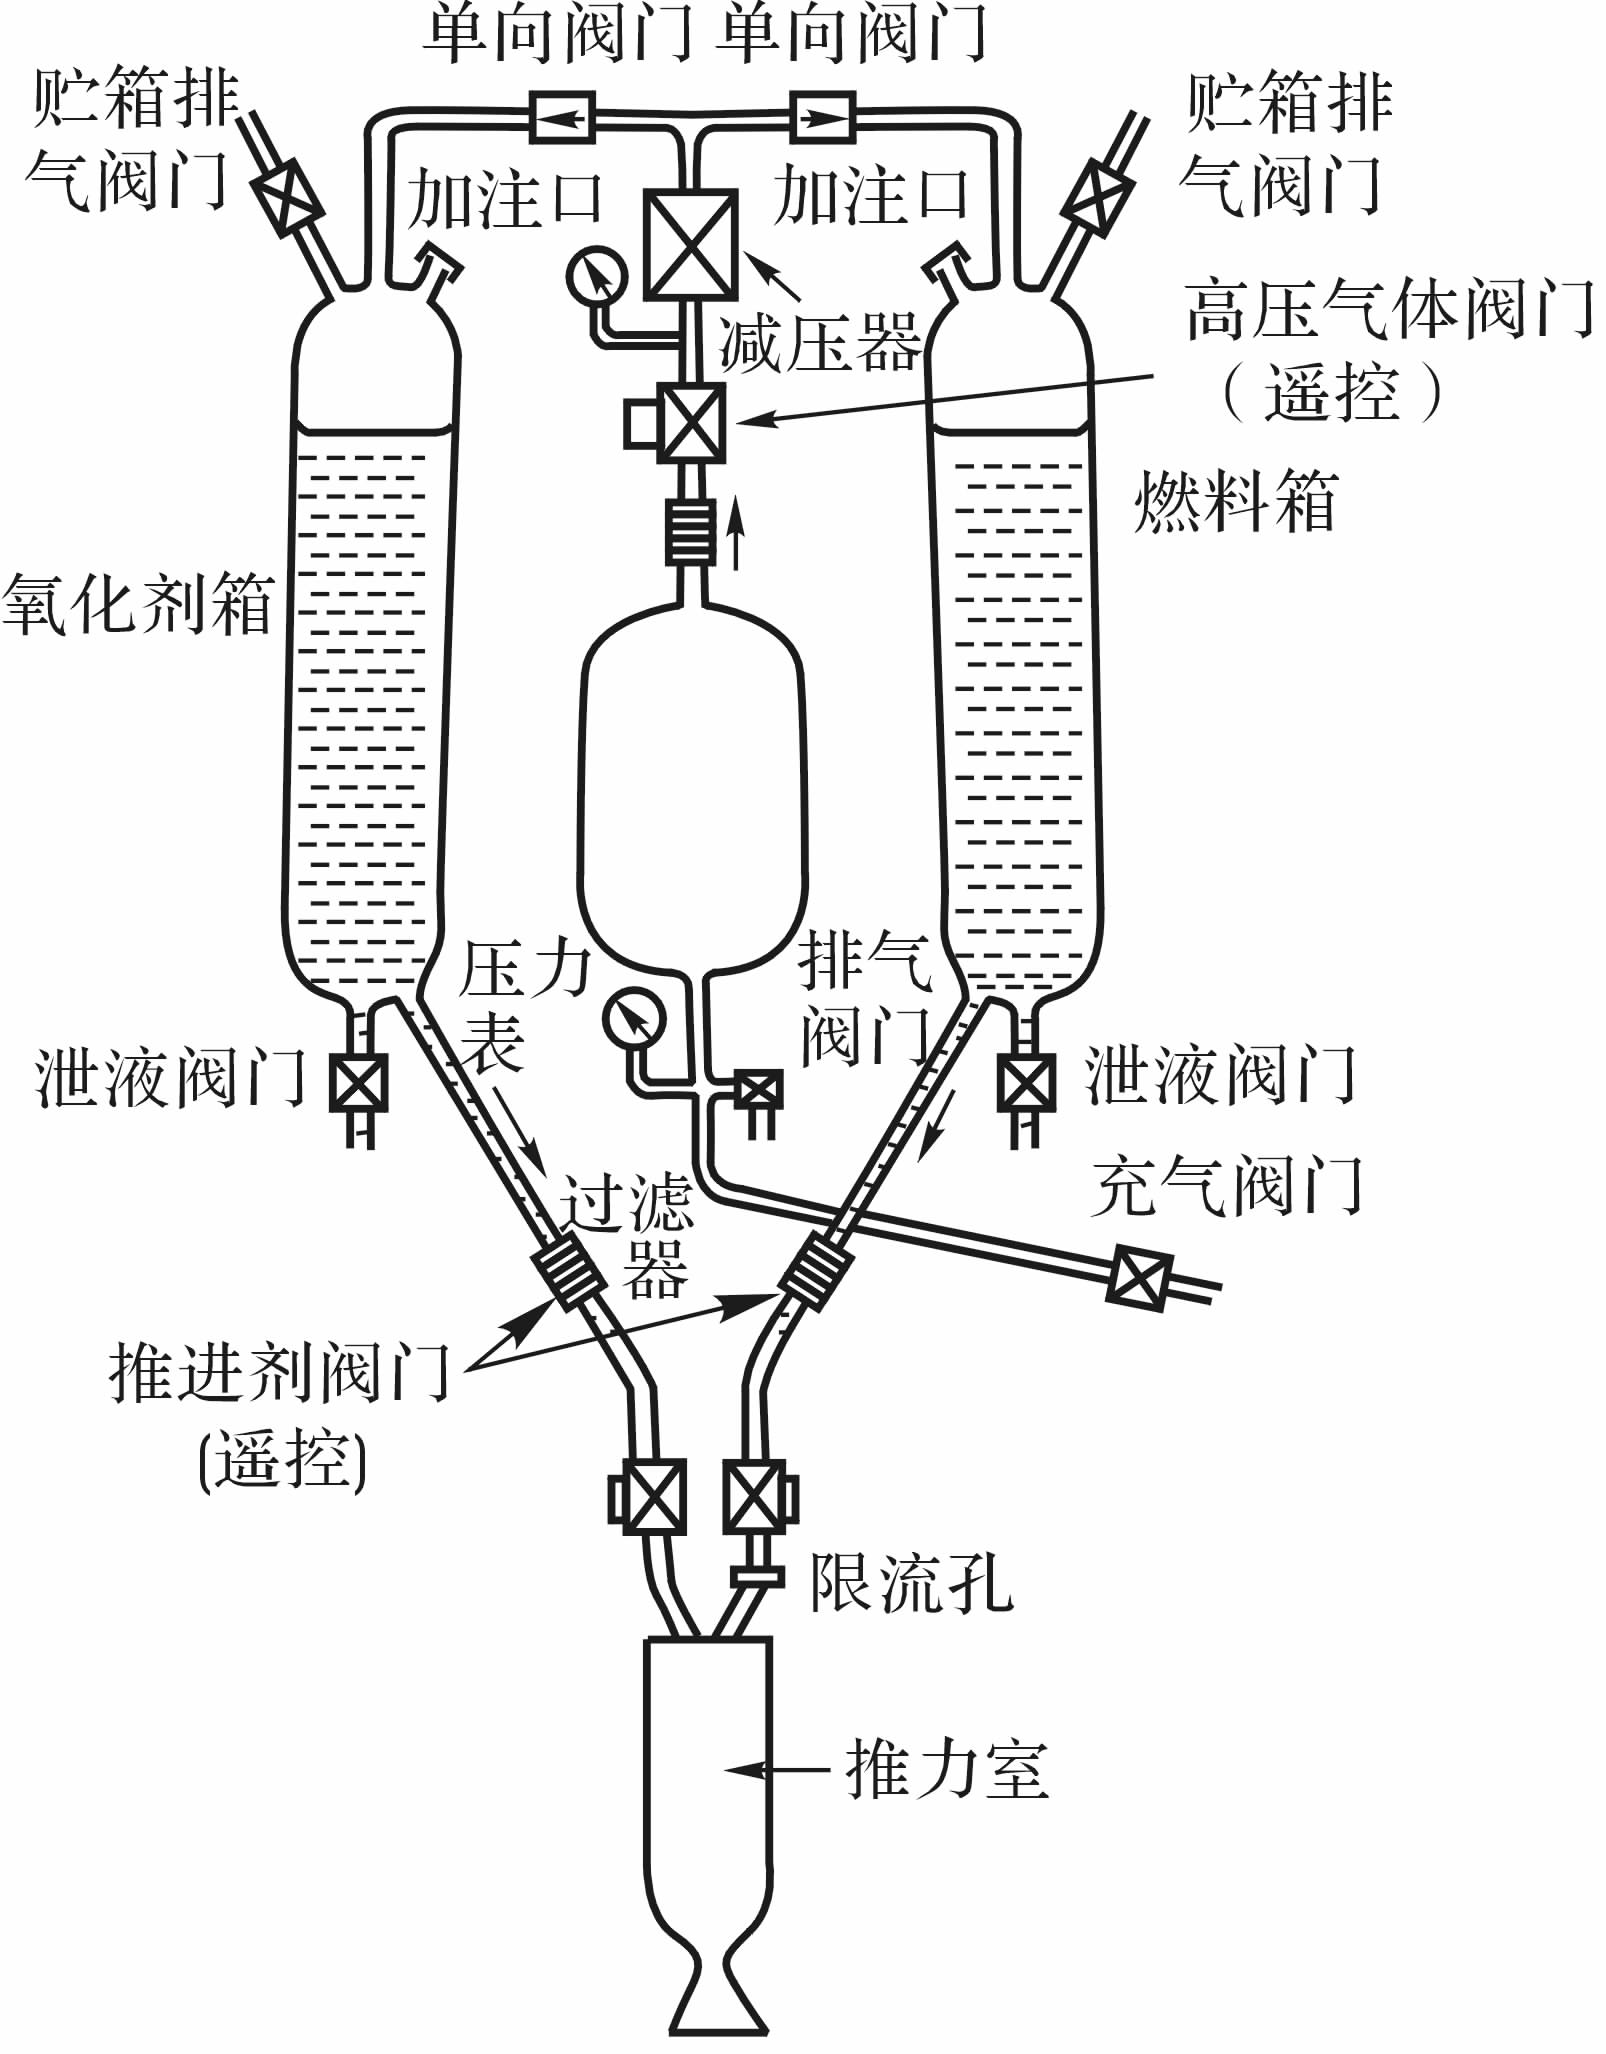
\includegraphics[width=0.8\linewidth]{pic/气压.png}
	\captionof{figure}{气体挤压式推进剂供应系统}
\end{minipage}


\vspace*{0.8em}
\noindent
\begin{minipage}{0.6\linewidth}
	\sssection[挤压式供应系统分类]
	
	\blue[对挤压工质的要求]\quad 与推进剂有良好的\red[相容性] ;最小的分子量具有适当的温度,且热稳定性要好。
	
	\hspace*{2em} 挤压气源是来自高压气瓶,瓶内压强约为20$\, \sim \,$35 MPa ,通过降压方式到工作压强。按照降压方式,又分为减压器降压式和直接膨胀降压式。
	\vspace*{0.8em}
	
	\sssection[冷气体挤压]
	\vspace*{-0.8em}
	\begin{enumerate}[\hspace*{1.5em} (1) ]
		\item \textbf{气瓶式(或贮气式)冷气挤压}\\
		\blue[常用挤压气体] \quad 空气、氮气和氦气。对于低温推进剂,空气和氮气遇冷后会发生凝结,应选用氦气。\vspace*{-0.5em}
		
		\item \textbf{蒸发系统汽化式}\\
		挤压气源是利用液体的汽化而得到。\\[0.5em]
		按照使用液体的来源,分为推进剂蒸发系统和非推进剂蒸发系统,即将容易气化的推进剂组元或非推进剂液体通过换热器加热、气化后去挤压贮箱中的推进剂。
		\begin{equation*}
			\begin{cases}
				\, \mbox{\blue[推进剂蒸发系统]}\quad \mbox{仅适用于热稳定的低沸点推进剂,如氢;(注:也适用泵式发动机)}\\
				\, \mbox{\blue[非推进剂蒸发系统]} \quad \mbox{主要是惰性气体蒸发系统,如液氮、液氦}
			\end{cases}
		\end{equation*}
	\end{enumerate}
\end{minipage}
\begin{minipage}{0.4\linewidth}
	\centering
	\vspace*{-4em}
	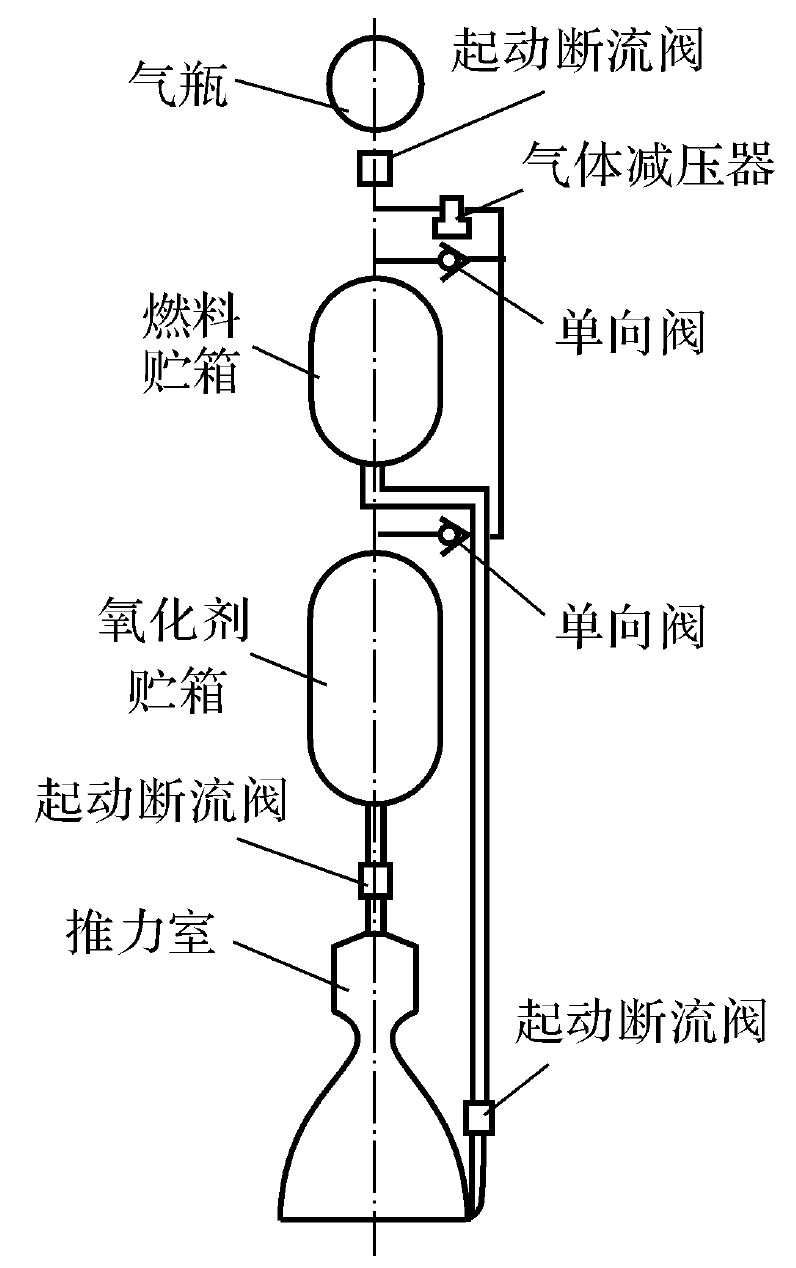
\includegraphics[width=0.8\linewidth]{pic/气瓶挤压.png}
	\vspace*{-1em}
	\captionof{figure}{气瓶式挤压式推进剂供应系统}
\end{minipage}

\vspace*{1em}
\sssection[热气体挤压]

\blue[适用范围] \quad 不能应用于低温推进剂:产物中的水会凝结吸热,会提高低温推进剂的温度。
\vspace*{0.5em}

\blue[分类]\quad 按产生热挤压气体的途径分类:
$
\begin{cases}
	\, \mbox{燃气发生器式}\\
	\, \mbox{化学反应式}
\end{cases}
$

\begin{enumerate}[\hspace*{1.5em} (1) ]
	\item \textbf{燃气发生器}\\
	按使用推进剂分类:
	\vspace*{-0.5em}
	\begin{enumerate}
		\item 固体燃气发生器\\
		基本组成\quad 固体推进剂燃气发生器(壳体、药柱、点火器)、过滤器和燃气调节装置及冷却热燃气的装置(不是必须)等。
		\begin{table}[!htb]
			\centering
			\setlength{\tabcolsep}{14mm}{
			\begin{tabular}{cl}
				\toprule
				固体燃气发生器类型 & 基本原理\\
				\midrule
				\makecell[c]{无冷却的\\固体燃气发生器} & \makecell[l]{固体燃气发生器产生燃气;\\过滤器过滤燃气;\\调节器排出多余燃气。}\\
				\hline
				 \makecell[c]{使用固体冷却剂的\\燃气发生器
} &\makecell[l]{推进剂:硝酸铵基;  冷却剂:粒状的草酸。 \\热燃气通过固体冷却剂冷却升华\\或分解产生附加的挤压气体($\text{CO}_2, \text{H}_2\text{O}, \text{CO}$)。}\\
				 \hline
				 \makecell[c]{使用叠氮化物冷却的\\燃气发生器} & \makecell[l]{热燃气通过叠氮化物冷却层被冷却,\\叠氮化物分解并产生氮气;\\但燃气中含有金属粒子,要用旋转分离除去。\\能提供较纯的氮气。
				 }\\
				 \hline
				 \makecell[c]{使用燃气发生器\\加热的氮气系统
} & \makecell[l]{固体燃气发生器安装在氦气瓶内,\\提供热量和 附加的挤压气体。
}\\
				\bottomrule
			\end{tabular}
		}
		\end{table}
	
	\begin{figure}[!htb]
		\begin{minipage}{0.25\linewidth}
			\centering
			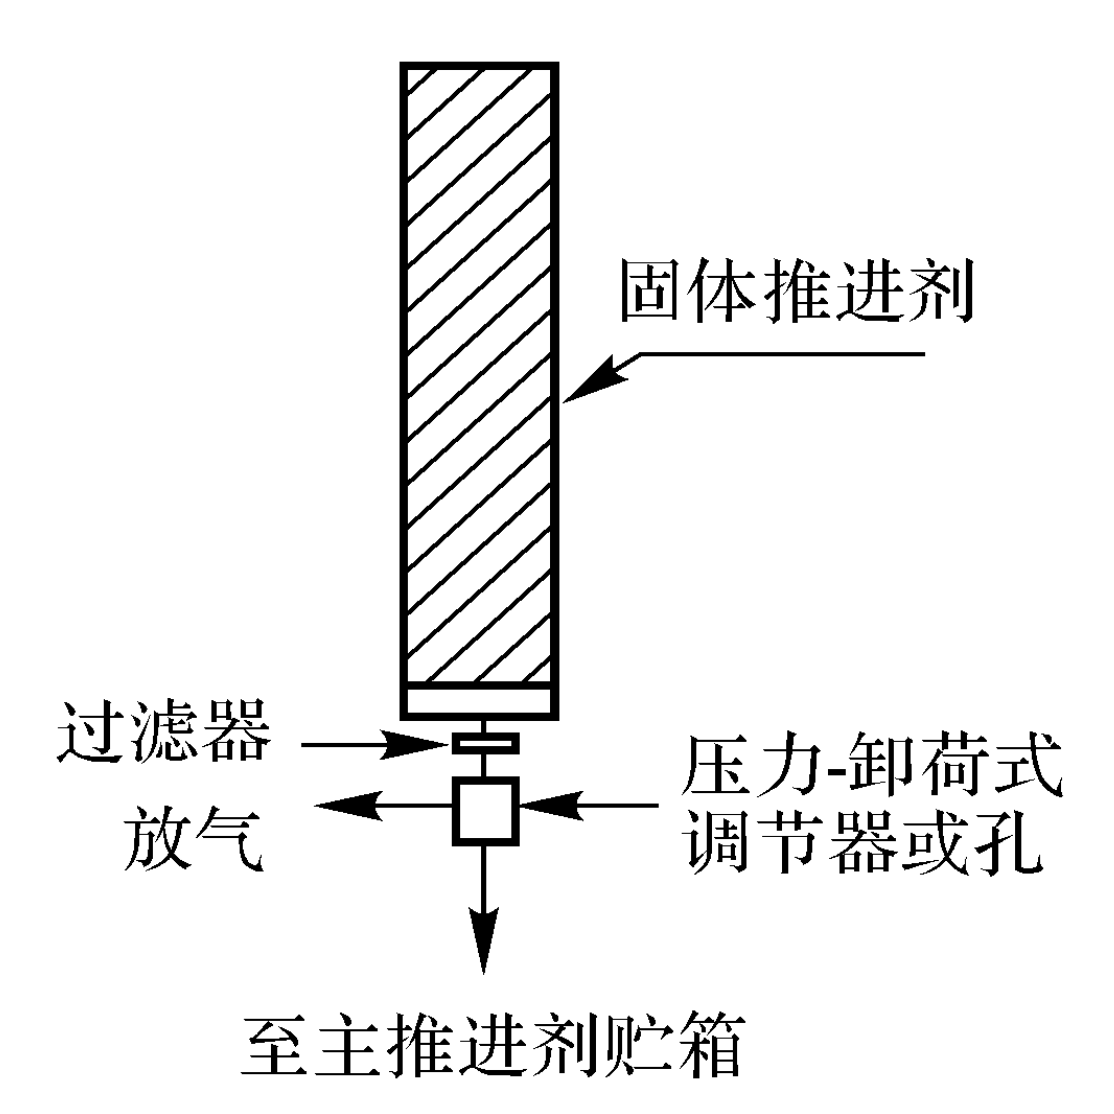
\includegraphics[width=\linewidth]{pic/固体1.png}
		\end{minipage}
		\begin{minipage}{0.25\linewidth}
			\centering
			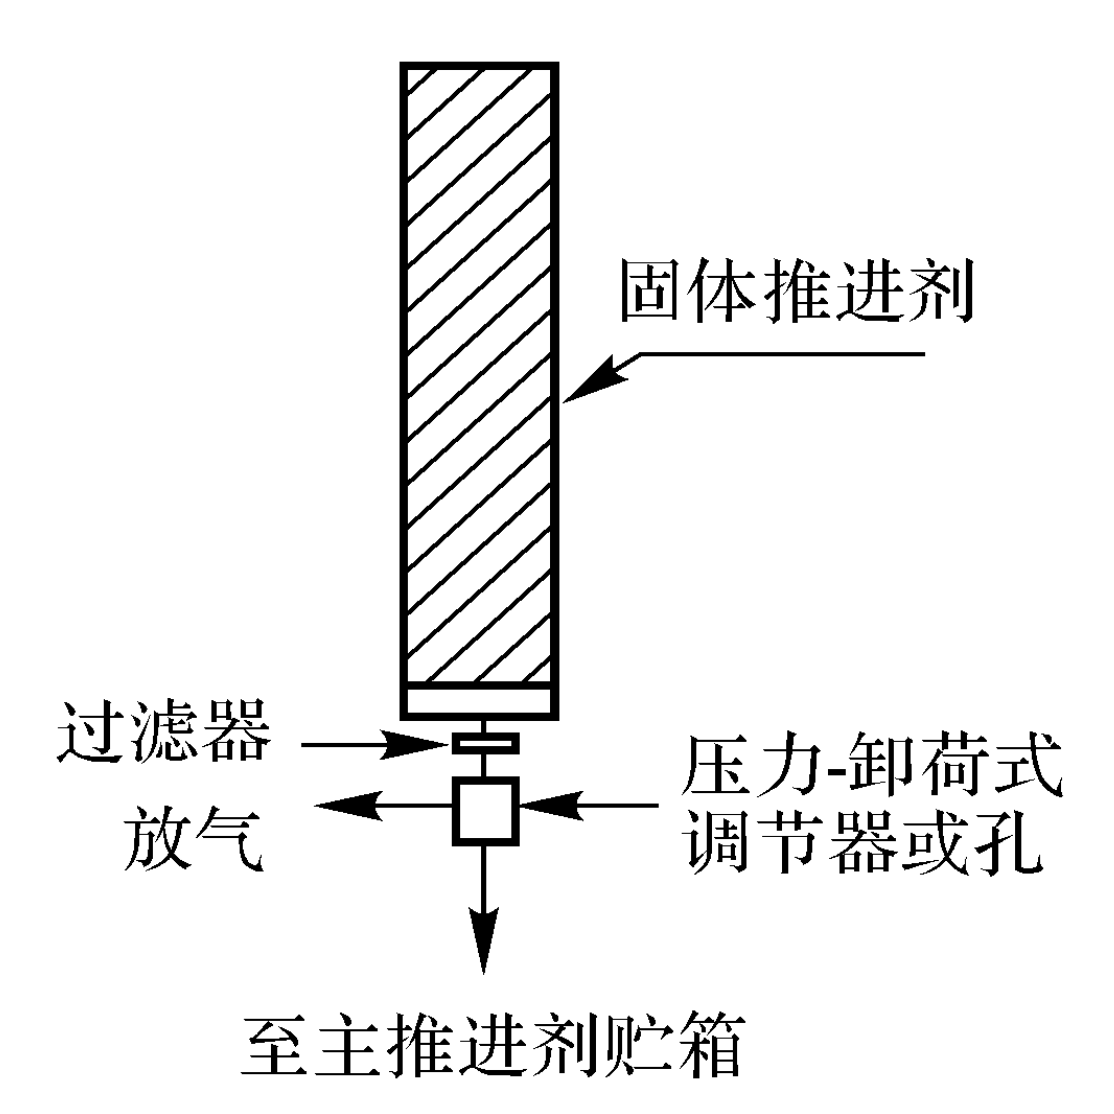
\includegraphics[width=\linewidth]{pic/固体1.png}
		\end{minipage}
		\begin{minipage}{0.25\linewidth}
			\centering
			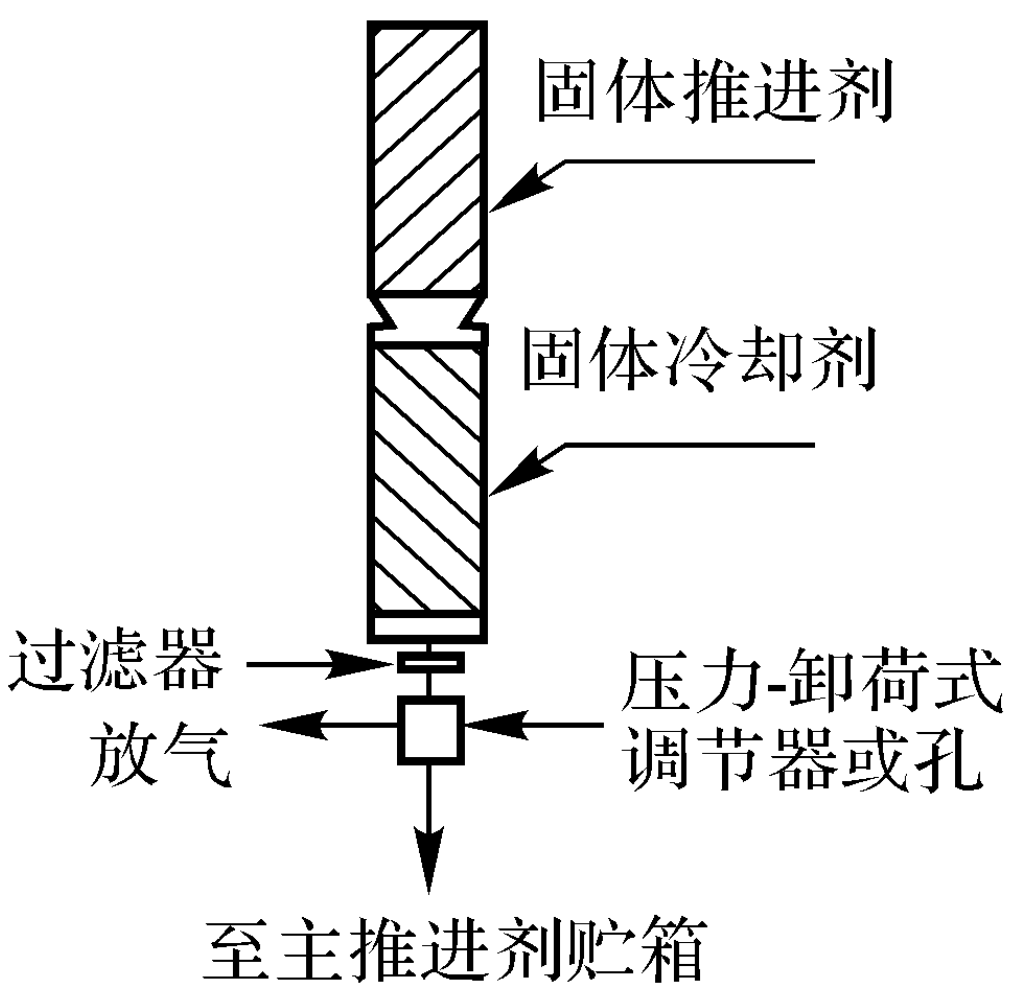
\includegraphics[width=\linewidth]{pic/固体3.png}
		\end{minipage}
		\begin{minipage}{0.20\linewidth}
			\centering
			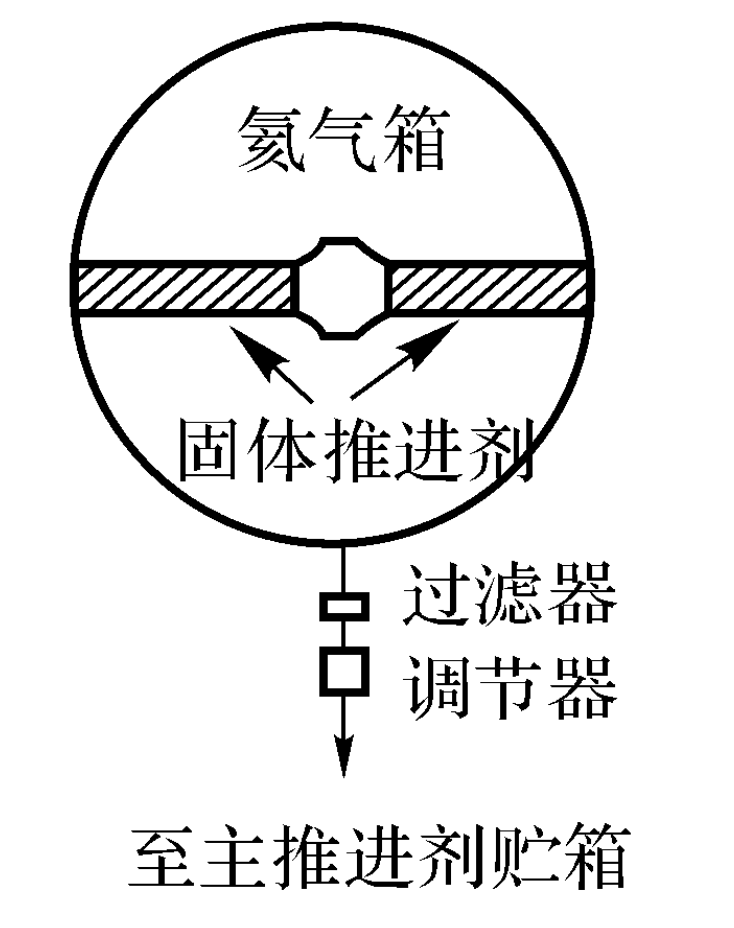
\includegraphics[width=\linewidth]{pic/固体4.png}
		\end{minipage}
	\caption{四种固体燃气发生器类型}
	\end{figure}
	
	\item 液体燃气发生器
	\begin{table}[!htb]
		\centering
		\setlength{\tabcolsep}{10mm}{
			\begin{tabular}{cl}
				\toprule
				液体燃气发生器类型 & 基本原理\\
				\midrule
				\makecell[c]{具有喷注冷却的\\单燃气发生器} & \makecell[l]{单组元$+$不反应的冷却剂, 产生低温燃气;\\
				双组元,使混合比远远偏离化学当量比,产生低温燃气。}\\
				\hline
				\makecell[c]{具有单个燃气\\发生器的氦气系统
} &\makecell[l]{燃气发生器通过换热器加热氦气,\\用热氦气其挤压 氧化剂贮箱;
\\燃气挤压主燃料贮箱。}\\
				\hline
				\makecell[c]{具有喷注冷却的\\两个双组元燃气发生器} & \makecell[l]{用氦气挤压两个辅助推进剂贮箱,供应燃气发生器;
\\富燃燃气发生器产生的燃气挤压主燃料贮箱;\\
富氧的燃气发生器产生的燃气挤压主氧化剂贮箱。}\\
				\bottomrule
			\end{tabular}
		}
	\end{table}
	
	典型的双组元液体燃气发生器式挤压系统如图\ref{双组元}所示。
	\end{enumerate}
	
	\begin{figure}[!htb]
		\centering
		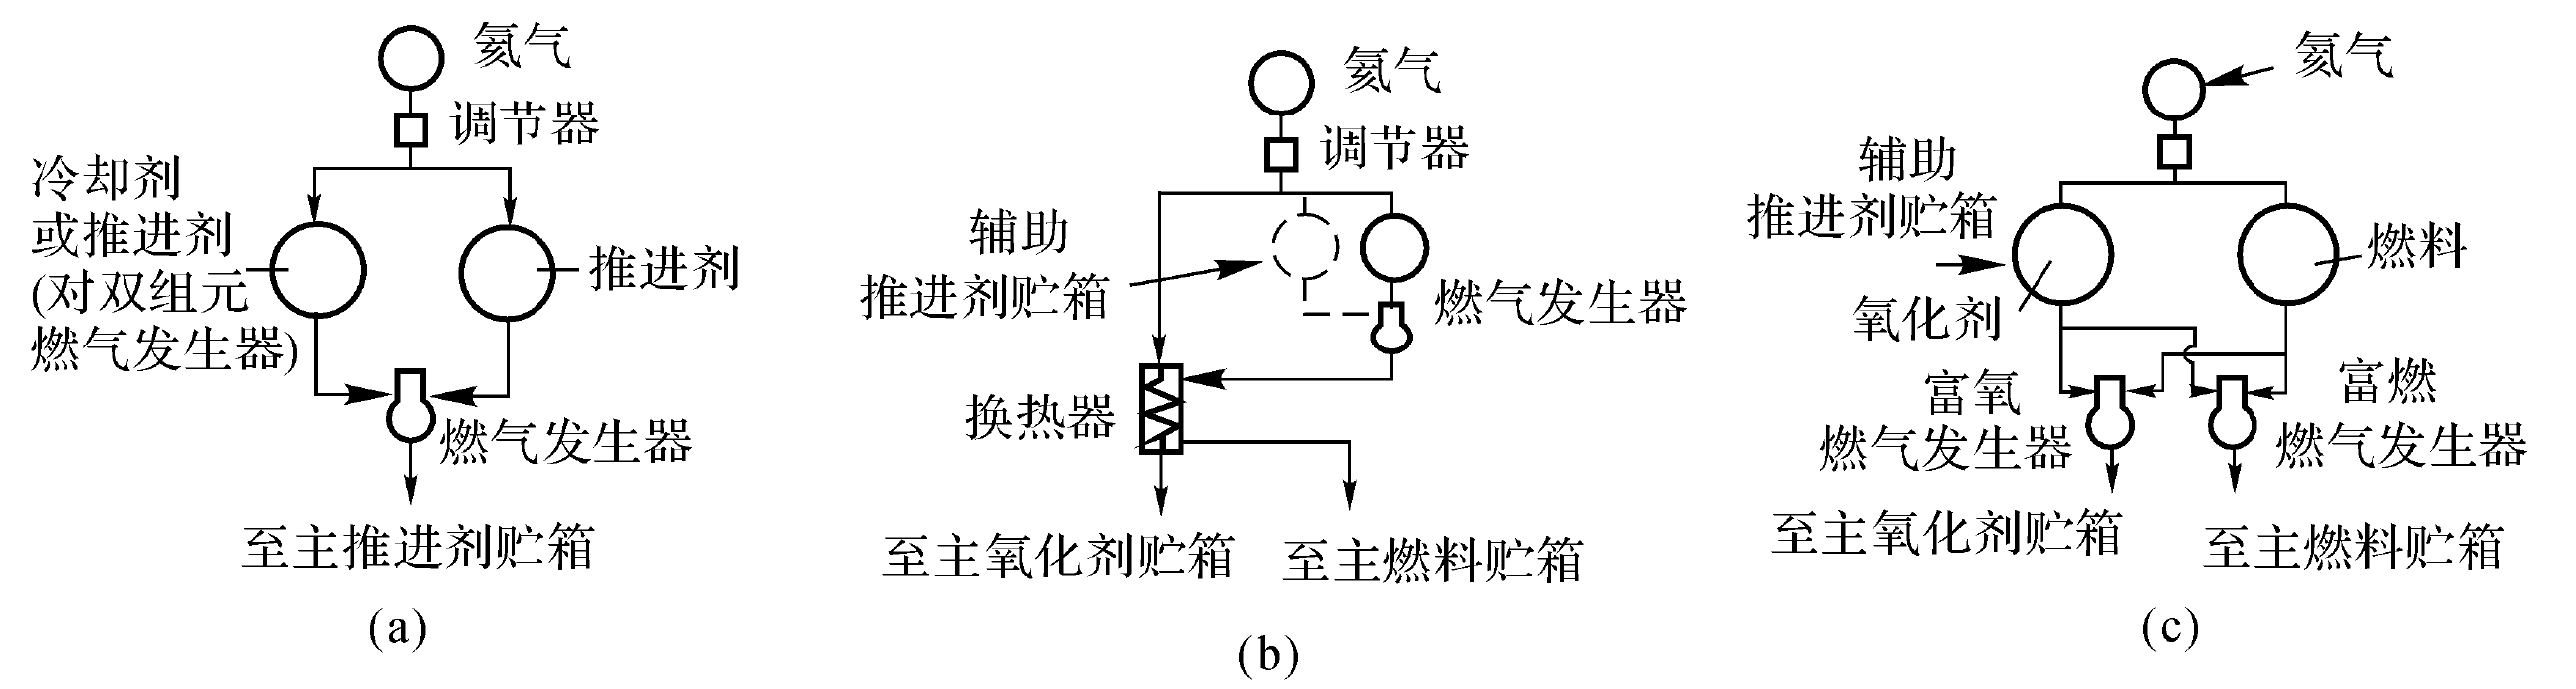
\includegraphics[width=0.9\linewidth]{pic/液体.png}
		\caption{三种液体燃气发生器类型}
	\end{figure}
	
	\begin{figure}[!htb]
		\centering
		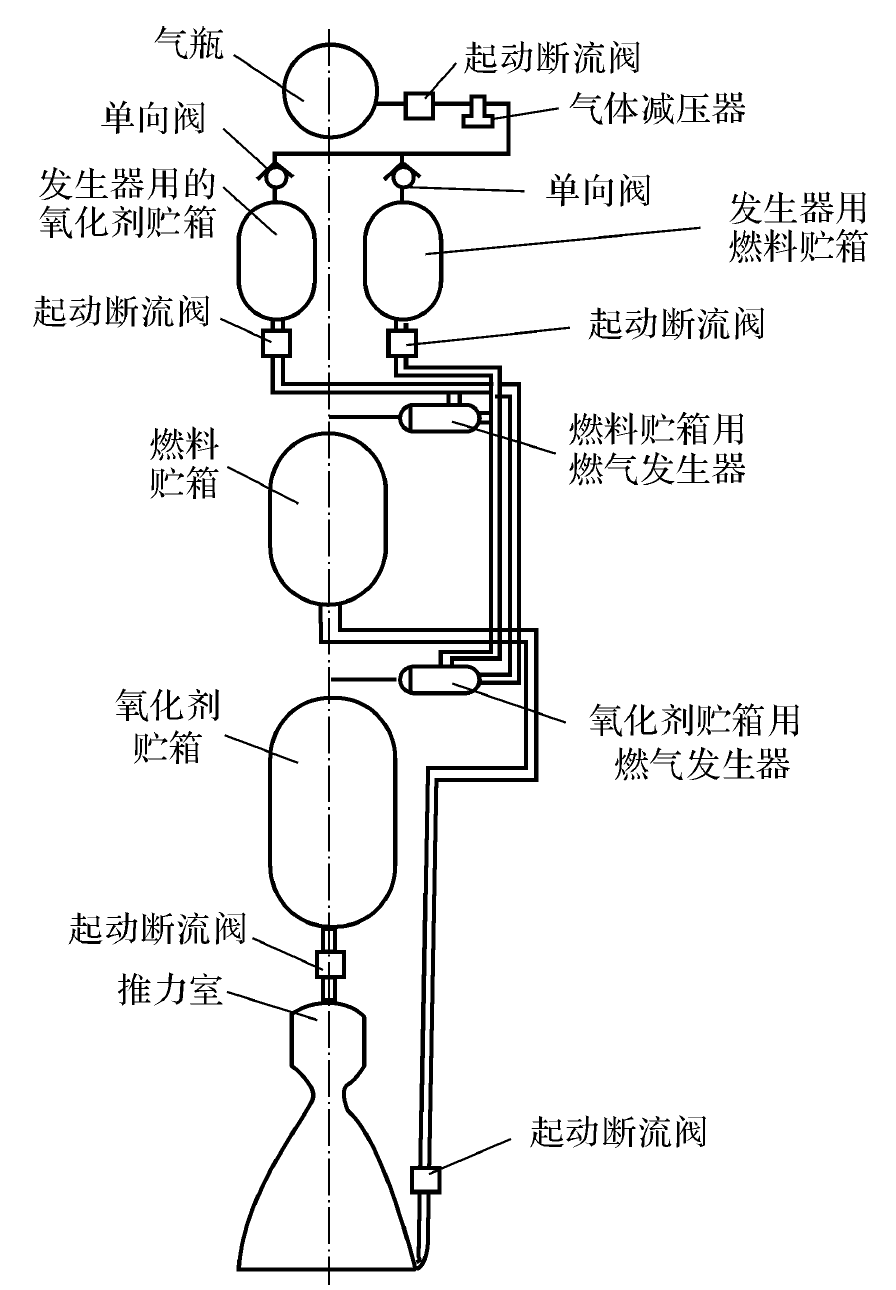
\includegraphics[width=0.35\linewidth]{pic/双组元液体.png}
		\caption{双组元液体燃气发生器式挤压系统}
		\label{双组元}
	\end{figure}
	
	\item \textbf{化学反应式}\\
	在贮箱中直接发生化学反应,即将少量燃料喷注到氧化剂贮箱中,或
将少量氧化剂喷注到燃料贮箱中,发生化学反应,从而产生挤压气体。
有两种类型:
	\vspace*{-0.5em}
	\begin{itemize}
		\item \blue[双直接喷注式]\quad 两个辅助贮箱。
		\item \blue[串联直接喷注式]\quad 一个辅助贮箱;在系统安全、可靠性和 调节贮箱稳态压力等方面存在设计问题。
	\end{itemize}
	\begin{figure}[!htb]
		\centering
		\subfigure[双直接喷注式]{
		\begin{minipage}{0.4\linewidth}
			\centering
			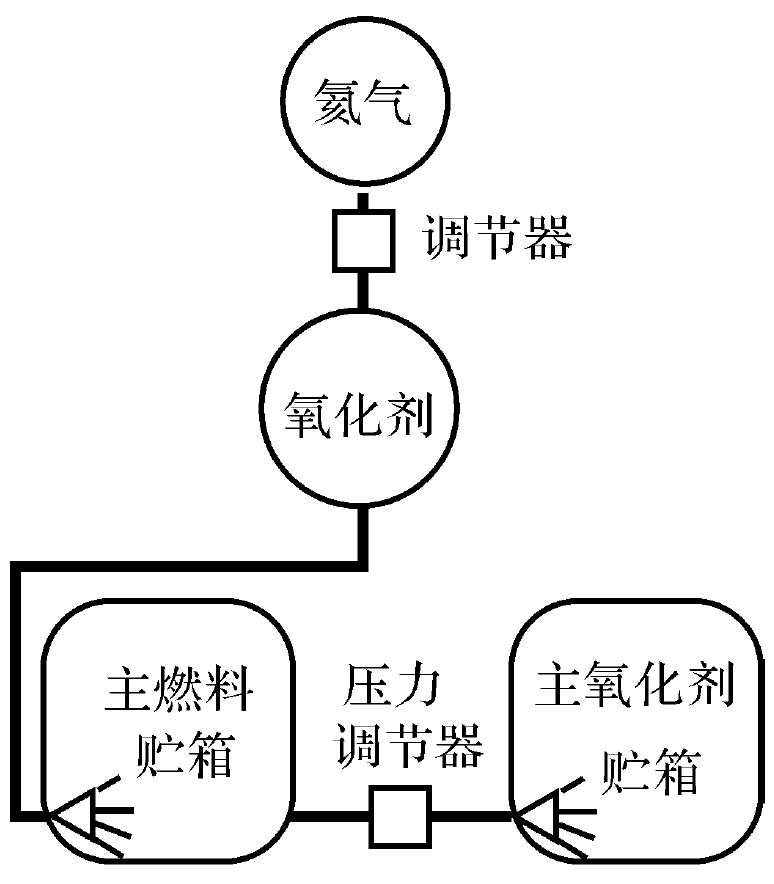
\includegraphics[width=0.5\linewidth]{pic/化学1.png}
			\vspace*{0.5em}
		\end{minipage}
		}
		\subfigure[串联直接喷注式]{
		\begin{minipage}{0.4\linewidth}
			\centering
			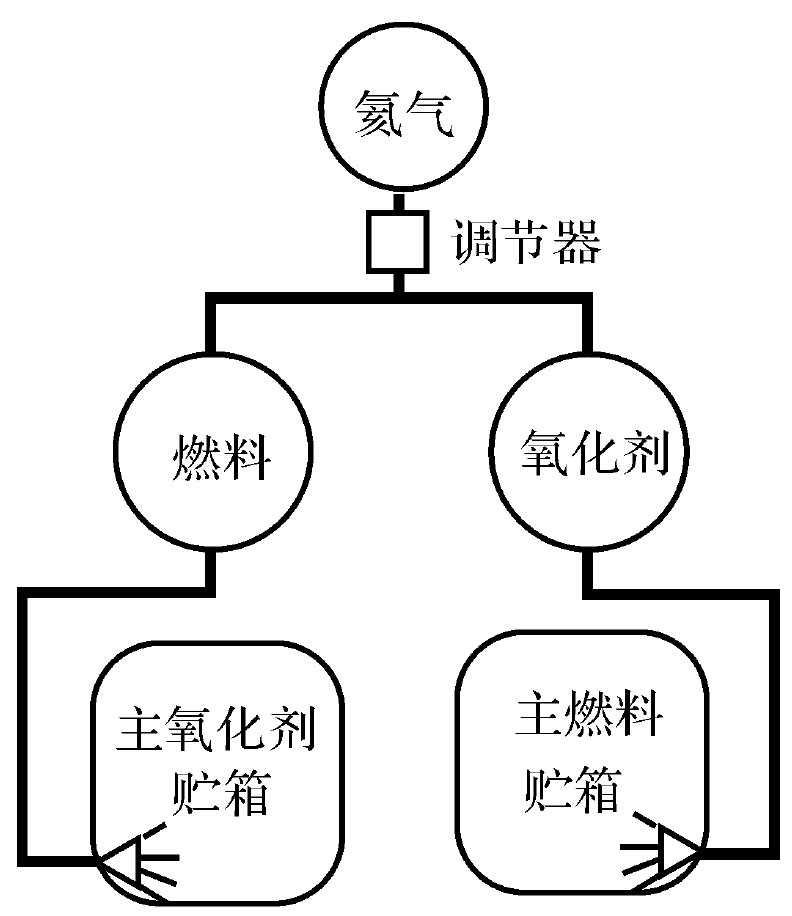
\includegraphics[width=0.5\linewidth]{pic/化学2.png}
			\vspace*{0.5em}
		\end{minipage}
	}
	\caption{化学反应式挤压系统}
	\vspace*{-2em}
	\end{figure}
\end{enumerate}

\sssection[各种挤压系统的对比]
\begin{table}[!htb]
	\centering
	\setlength{\tabcolsep}{2.5mm}{
	\begin{tabular}{m{0.1\textwidth}<{\centering} m{0.25\textwidth}<{\centering} m{0.25\textwidth}<{\centering} m{0.28\textwidth}<{\centering}}
		\toprule
		类别 & 气瓶贮气系统 & 液体蒸发系统 & 热气挤压系统 \\
		\midrule
		优点 & 结构简单,技术成熟 & 辅助气瓶和辅助贮箱尺寸小系统结构质量小 & 辅助气瓶和辅助贮箱尺寸小,系统结构质量小固体发生器系统结构简单\\
		\hline
		缺点 & 气瓶容积大,系统质量大 & 需要辅助气瓶、辅助贮箱和换热器,结构复杂 & 对液体发生器和在贮箱中直接化学反应的系统,结构复杂;固体发生器系统不能多次起动\\
		\hline
		适用范围 & 总冲量比较小的发动机 & 热稳定、低沸点的推进剂组元,若推进剂都不易汽化,可以选用液化气体 & 常温推进剂\\
		\bottomrule
	\end{tabular}
}
\end{table}

\noindent \textbf{\underline{挤压系统的选择}}

\par (1) \hspace*{0.5em}\red[任务和运载器的要求。]包括贮存性能、系统的起动和再起动以及压强和流量的精度等。
\par (2) \hspace*{0.5em}\red[挤压气体与推进剂、贮箱材料的相容性。] 包括化学惰性、过凝结和过溶解气体产物的防止以及适当的挤压物质温度。
\par (3) \hspace*{0.5em}\red[挤压式系统的可靠性。] 可靠性是在系统复杂性和失效模式的基础上估计的,应大力发展可靠性高的组件,包括燃气发生器、换热器和调节器等。
\par (4) \hspace*{0.5em}\red[成本。]
\par (5) \hspace*{0.5em}\red[挤压式系统的重量和尺寸。]

挤压系统的\blue[特点]:技术成熟,可靠性高;系统比较笨重。\blue[适用于]小推力或工作时间较短的火箭发动机。
\vspace*{0.5em}

\subsection{泵压式推进剂供应系统}

\begin{figure}[!htb]
	\centering
	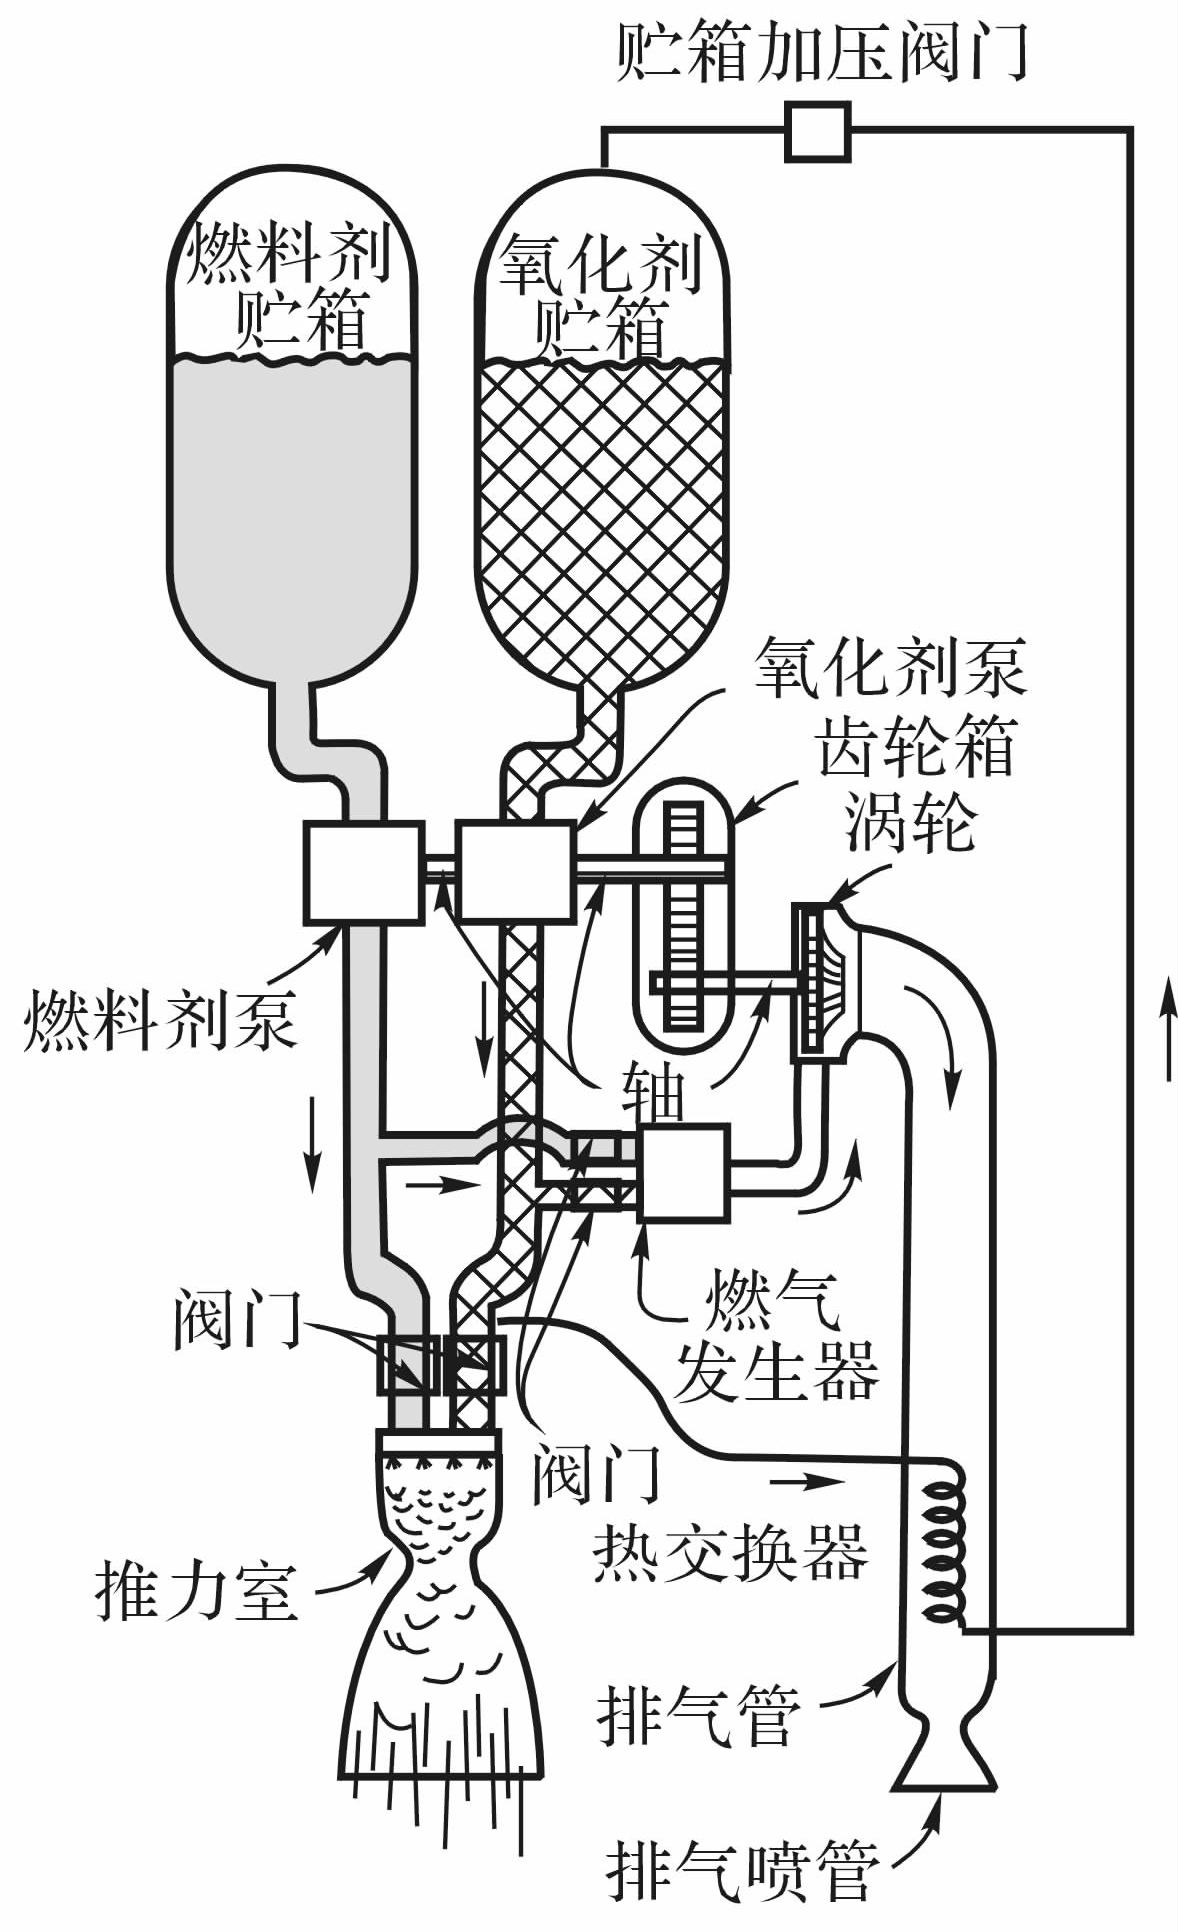
\includegraphics[width=0.3\linewidth]{pic/泵压.png}
	\caption{泵压式推进剂供应系统}
\end{figure}

\defination[泵压式供应系统]
{
	\blue[原理]\quad 利用涡轮泵将推进剂从贮箱中抽出、增压,输送至推力室;\\
	\hspace*{2em} \blue[关键部件]\quad 涡轮泵\\
	\hspace*{2em} \blue[特点]\quad 泵前推进剂是低压,贮箱结构质量可以较轻,一般$\le 0.5\,$MPa.\\
	\hspace*{2em} \blue[适用]\quad 工作时间长的大中型液体发动机。
}


\noindent \textbf{1. 泵压式系统的分类}

(1) \hspace*{0.5em} \dy[开式循环]{KSXH} \quad 驱动涡轮的工质气体经排气管直接排入周围环境,或者引入喷管下游与主燃气一起膨胀排出。
\begin{equation*}
	\mbox{开式循环}\,
	\begin{cases}
		\, \mbox{\dy[燃气发生器循环]{RQFSQXH}}\\
		\, \mbox{\dy[抽气循环]{CQXH}}
	\end{cases}
\end{equation*}

(2) \hspace*{0.5em} \dy[闭式循环]{BSXH} \quad 驱动涡轮的工质全部排入推力室,与燃烧室中的推进剂燃烧后,与主燃气一起从喷管排出。

\begin{equation*}
	\mbox{闭式循环}
	\, 
	\begin{cases}
		\, \mbox{\dy[膨胀循环]{PZXH}}\\
		\, \mbox{\dy[分级燃烧循环]{FJRSXH}(\dy[补燃循环]{BRXH})}
	\end{cases}
\end{equation*}

\vspace*{0.5em}

\noindent \textbf{2. 燃气发生器循环}

\defination[燃气发生器循环]
{
	\blue[原理]:驱动涡轮的工质气体是燃气发生器产生的燃气,\red[挤压式燃气发生器式生成的燃气用于挤压,泵压式燃气发生器生成的燃气用于驱动涡轮]。\\
	\hspace*{2em} \blue[工作条件]:燃烧室压强一般为$4 \, \sim \, 15\,$MPa,比冲下降$1\% \, \sim \, 5\%$。\\
	\hspace*{2em} \blue[分类]:单组元、双组元;\\
	\hspace*{2em} \blue[燃气温度]:燃气温度较低,以满足涡轮叶片的要求;\\
	\hspace*{2em} \blue[混合比]:通常在较高或者较低的混合比下工作,以生成低温的燃气;\\
	\hspace*{2em} \blue[优点]:系统简单,技术成熟;\\
	\hspace*{2em} \blue[缺点]:燃气直接排入环境,会造成发动机性能下降,室压增高损失增大。
}
{
	\begin{figure}[!htb]
		\centering
		\begin{minipage}{0.45\linewidth}
			\centering
			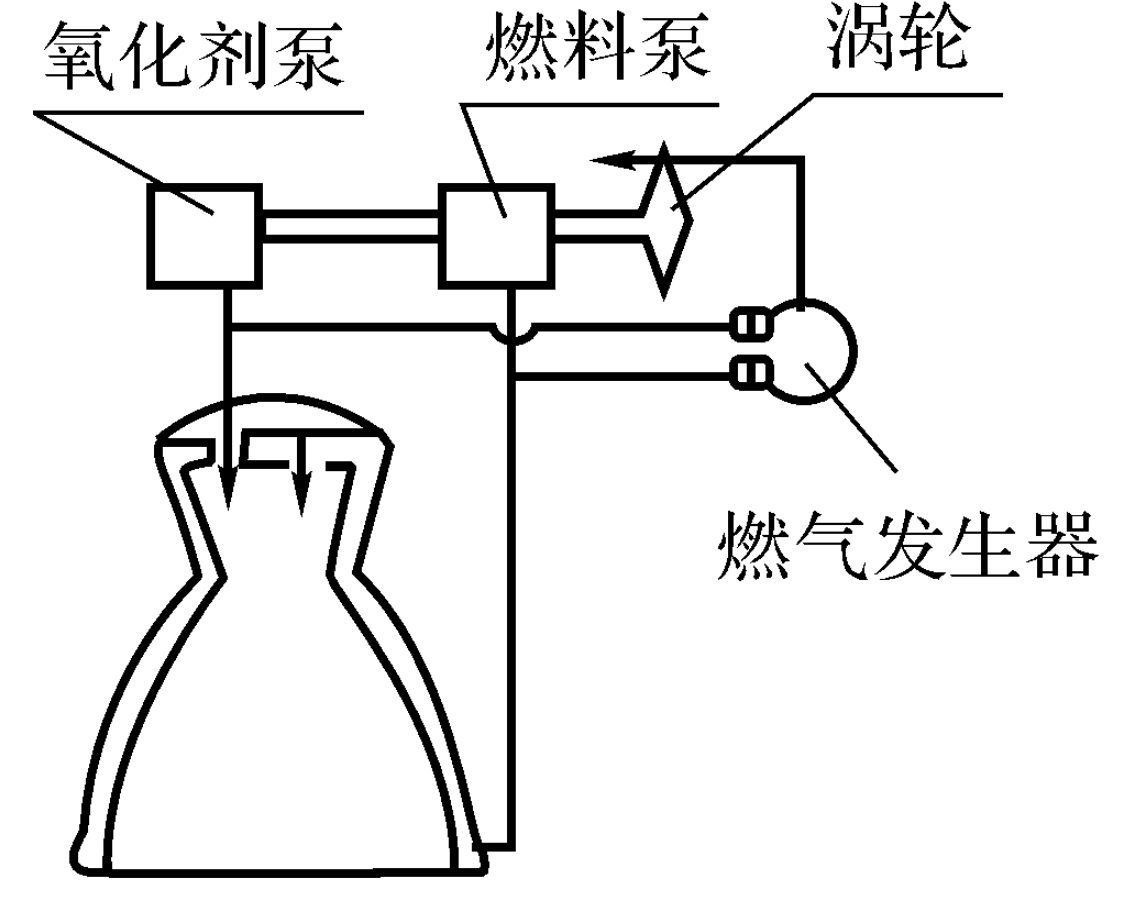
\includegraphics[width=0.67\linewidth]{pic/燃气发生器1.png}
			\caption{双组元燃气发生器}
		\end{minipage}
		\begin{minipage}{0.417\linewidth}
			\centering
			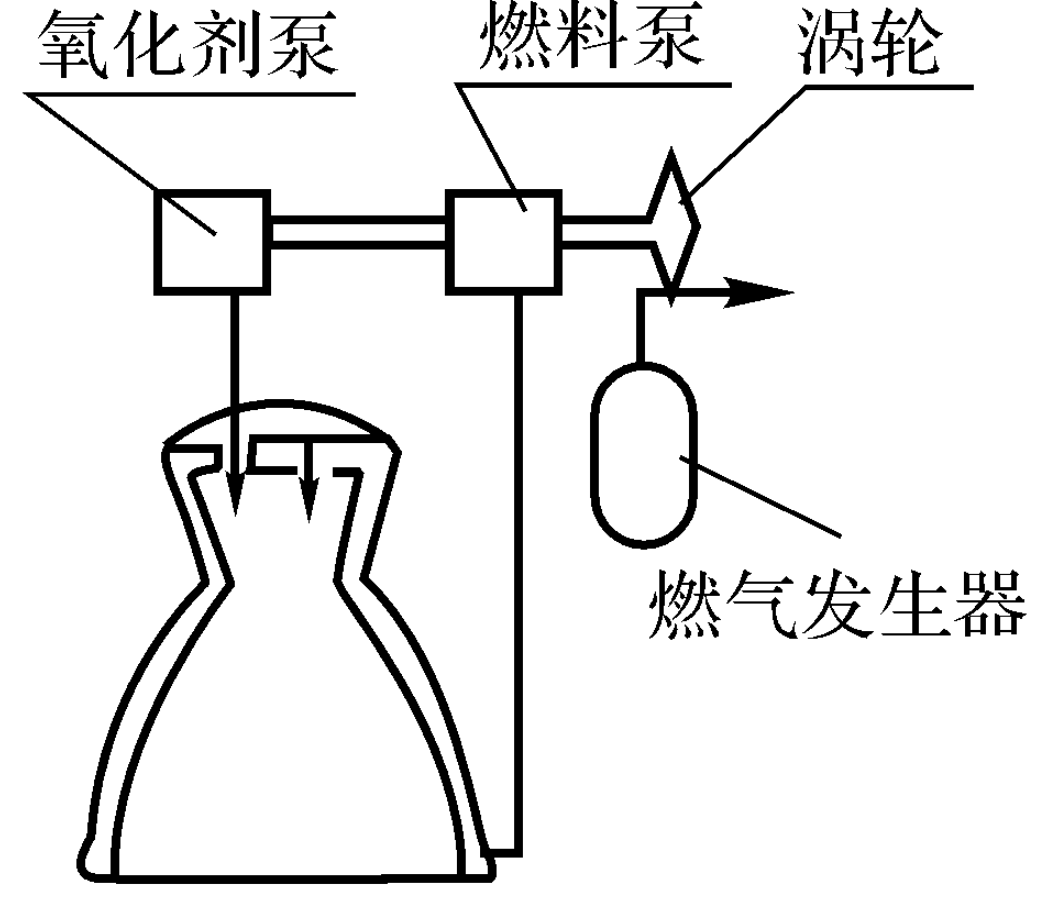
\includegraphics[width=0.667\linewidth]{pic/燃气发生器2.png}
			\caption{单组元燃气发生器}
		\end{minipage}
	\end{figure}
}

\vspace*{0.5em}

\noindent \textbf{3. 抽气循环}

\defination[抽气循环]
{
	\blue[原理]:开式循环,驱动涡轮工质气体是从燃烧室喷注面附近引出的燃气,此处引出的燃气温度较低,可使涡轮正常工作。\\
	\hspace*{2em} \blue[优点]:结构简单,质量较小;\\
	\hspace*{2em} \blue[缺点]:技术难度较大;有能量损失。
}

{
	\begin{figure}[!htb]
		\centering
		\begin{minipage}{0.45\linewidth}
			\centering
			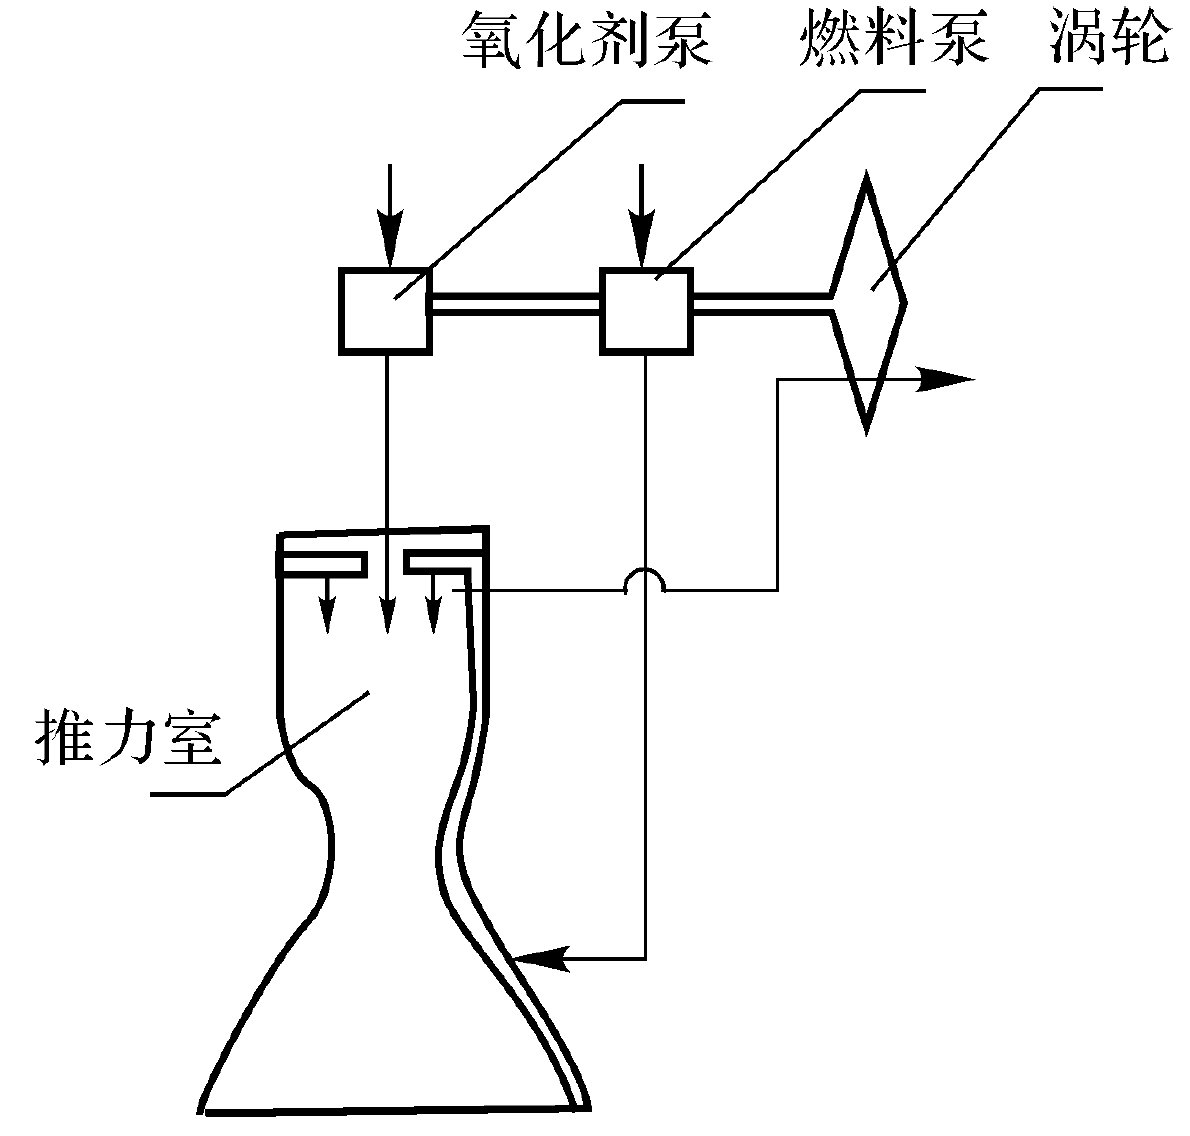
\includegraphics[width=0.7\linewidth]{pic/抽气循环.png}
			\caption{抽气循环}
		\end{minipage}
		\begin{minipage}{0.45\linewidth}
			\centering
			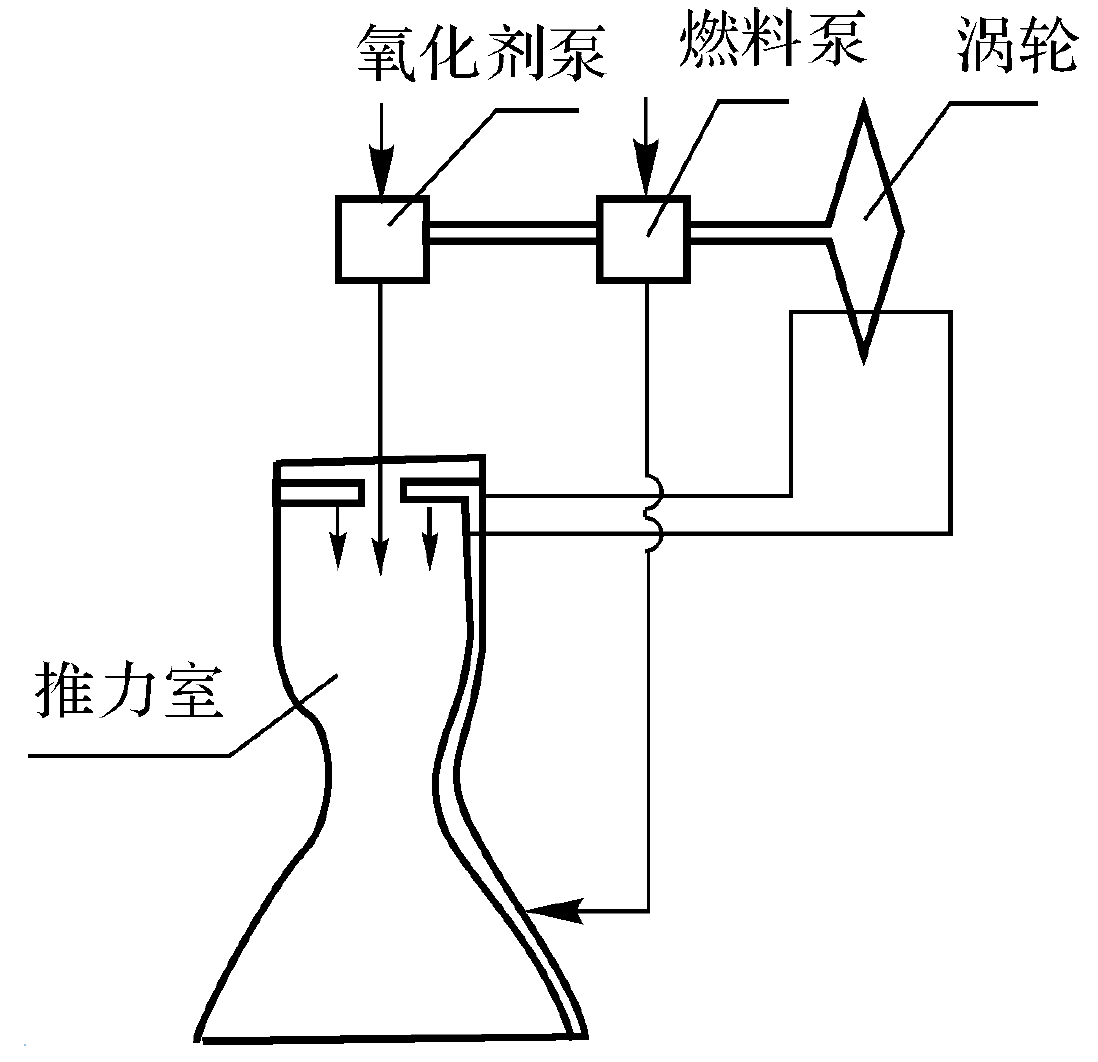
\includegraphics[width=0.682\linewidth]{pic/膨胀循环.png}
			\caption{膨胀循环}
		\end{minipage}
	\end{figure}
}

\noindent \textbf{4. 膨胀循环}

\defination[膨胀循环]
{
	\blue[原理]:闭式循环,将推力室冷却套中汽化和加热了的气态推进剂引出来驱动涡轮,从涡轮排除后再喷入推力室,与主推进剂燃烧后喷出。\\
	\hspace*{2em} \blue[工作条件]:燃烧室压强一般为$3 \, \sim \, 10\,$MPa, 对推进剂有要求,适用于液氢液氧发动机,且主要用于上面级。\\
	\hspace*{2em} \blue[优点]:可获得较高比冲,结构简单,质量轻,可靠性高;\\
	\hspace*{2em} \blue[缺点]:加热汽化的推进剂做功能力有限,高压强不适用。
}


{
	\begin{figure}[!htb]
		\centering
		\begin{minipage}{0.33\linewidth}
			\centering
			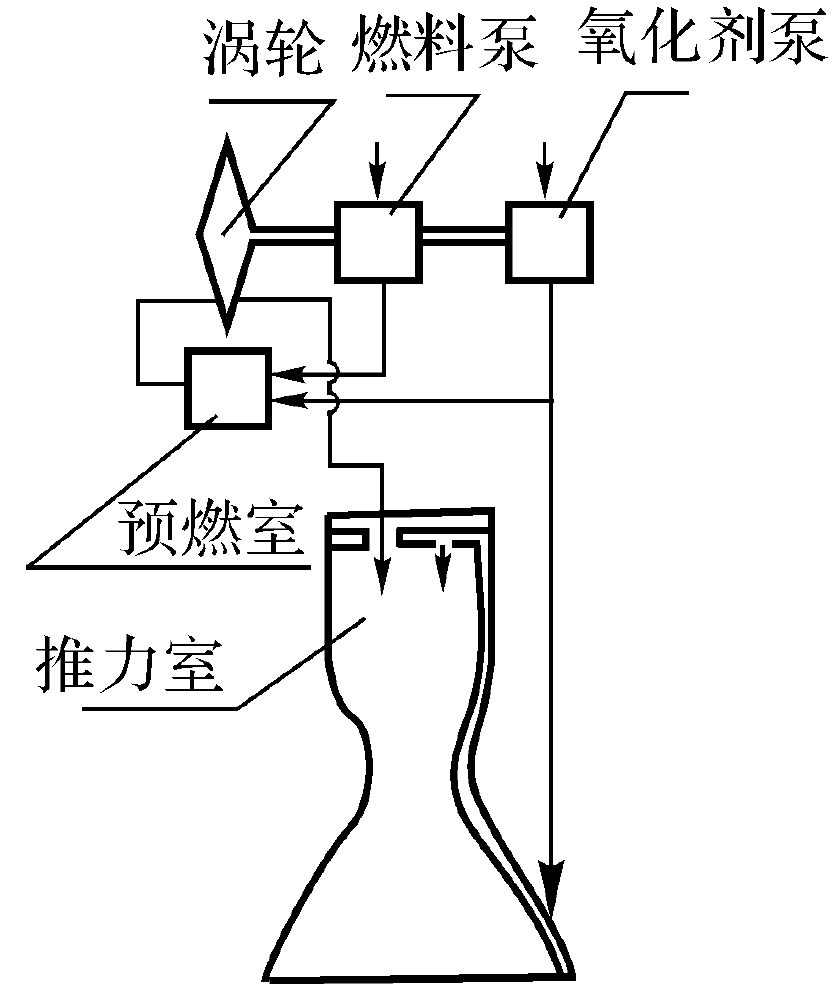
\includegraphics[width=0.9\linewidth]{pic/富燃顶燃.png}
			\caption{富燃顶燃室}
		\end{minipage}
		\begin{minipage}{0.33\linewidth}
			\centering
			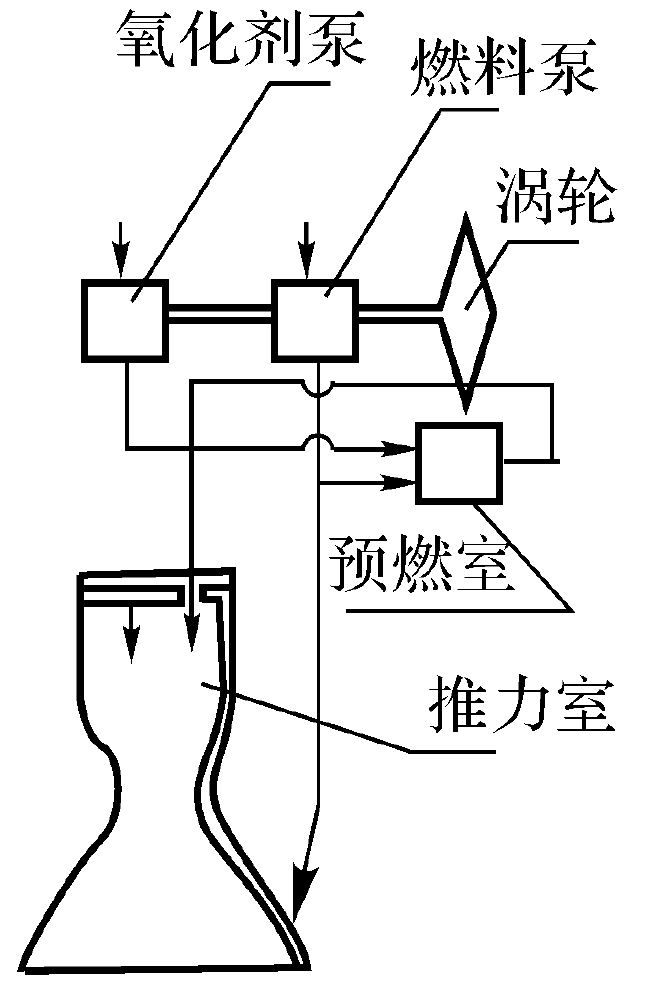
\includegraphics[width=0.695\linewidth]{pic/富燃预燃.png}
			\caption{富燃预燃室}
		\end{minipage}
		\begin{minipage}{0.33\linewidth}
			\centering
			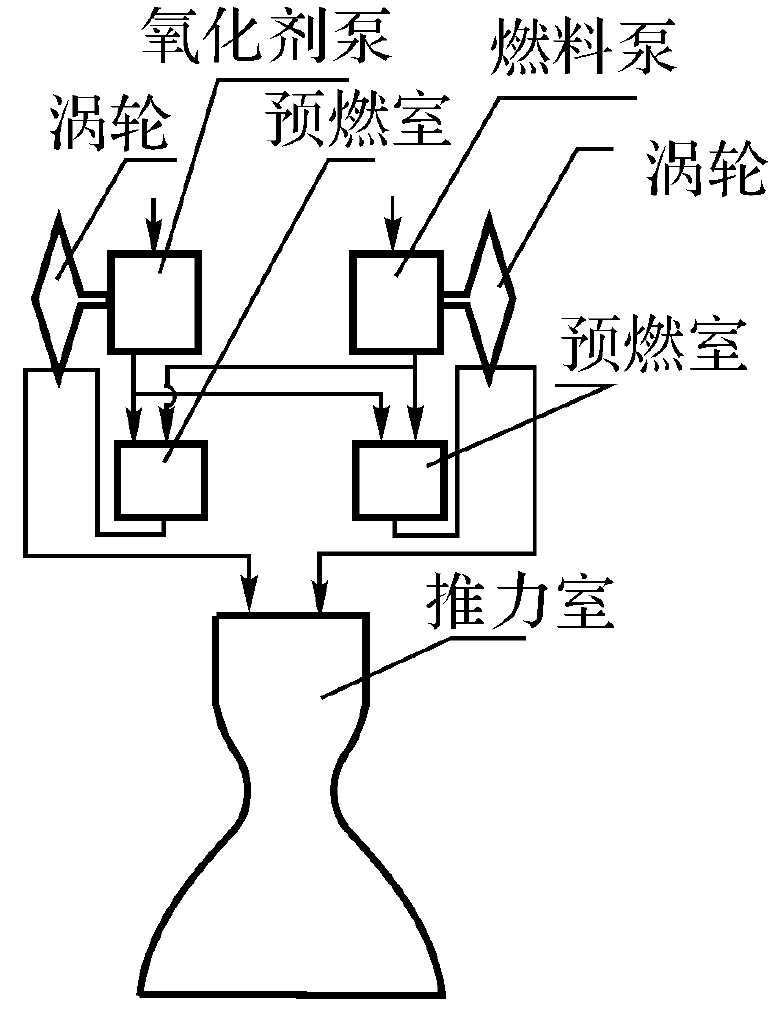
\includegraphics[width=0.82\linewidth]{pic/双预燃.png}
			\caption{双预燃室}
		\end{minipage}
	\end{figure}
}

\clearpage

\noindent \textbf{5. 分级燃烧循环(补燃循环)}

\defination[分级燃烧循环(补燃循环)]
{
	\blue[原理]:闭式循环,将一种推进剂组元的全部流量和另一种推进剂组元的部分流量输送到预然室中燃烧,产生低温燃气驱动涡轮,从涡轮排出的燃气再喷入推力室中进行补燃;\\
	\hspace*{2em} \blue[特点]:涡轮工质流量大,输出的功率大,燃烧室压力高,可获得最高
的发动机比冲;\\
	\hspace*{2em} \blue[全流量补燃循环]:将两种推进剂组元的全部流量输送到预燃室进行燃烧的循环。\\
	\hspace*{2em} \blue[分类]:富燃预燃室、富氧预燃室、双预燃室。
}

\noindent \textbf{6. 各种循环的优缺点和使用范围}
\begin{table}[!htb]
	\centering
	\setlength{\tabcolsep}{3.6mm}{
		\begin{tabular}{m{0.07\textwidth}<{\centering} m{0.25\textwidth} m{0.16\textwidth} m{0.15\textwidth} m{0.15\textwidth}}
			\toprule
			\makecell[c]{种类} & \makecell[c]{燃气发生器循环} & \makecell[c]{抽气循环}& \makecell[c]{抽气循环} & \makecell[c]{补燃循环} \\
			\midrule
			优点 & 结构简单,质量轻,有研制经验,推力和混合比易调节,推力工作范围较宽 & 结构简单,质量轻 & 比冲高,结构简单,涡轮工质清洁 & 比冲高,极限室压高\\
			\hline
			缺点 & 比冲低,燃烧室压强高时比冲损失大 & 推力室设计复杂,抽出的燃气需降温和调节,比冲低 & 燃烧室压强高时不适用,启动加速慢 & 结构复杂,质量大,性能参数调节和校准困难\\
			\hline
			推进剂 & 种类不受限制,发生器和推力室可以使用相同推进剂 & 推进剂种类不受限制 & 主推进剂的一种组元必须易气化,且分子量小 &种类不受限制,特别适用液氢液氧 \\
			\hline
			推力室\newline 和室压 & 单组元方案适用于低推力和低室压;双组元方案推力不受限;高室压比冲损失大,室压有上限 & 推力不受限制,室压有上限 & 适用于较低推力和室压 & 推力不受限制,适用于高室压 \\
			\hline
			比冲 & 低 & 低 & 高 & 高\\
			\bottomrule
		\end{tabular}
	}
\end{table}

\begin{figure}[!htb]
	\centering
	\begin{minipage}{0.49\linewidth}
		\centering
		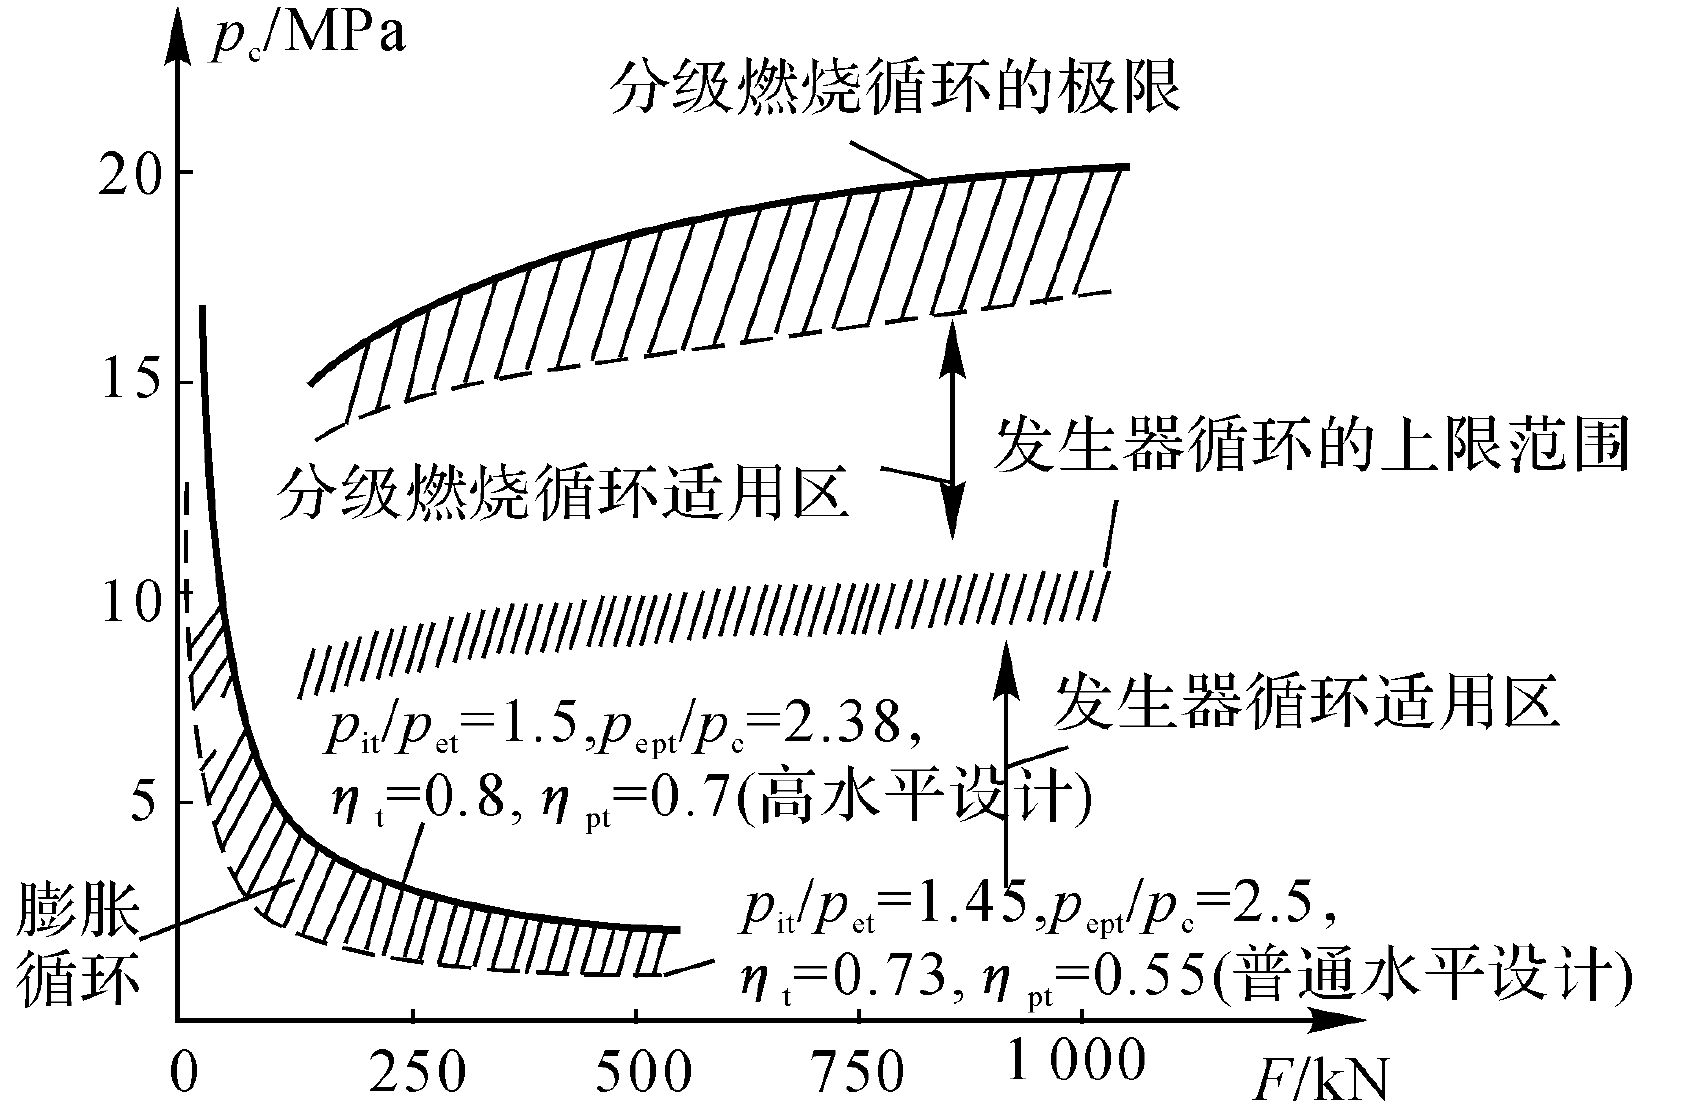
\includegraphics[width=\linewidth]{pic/三循环使用范围.png}
		\caption{三种循环的使用范围比较}
	\end{minipage}
	\begin{minipage}{0.49\linewidth}
		\centering
		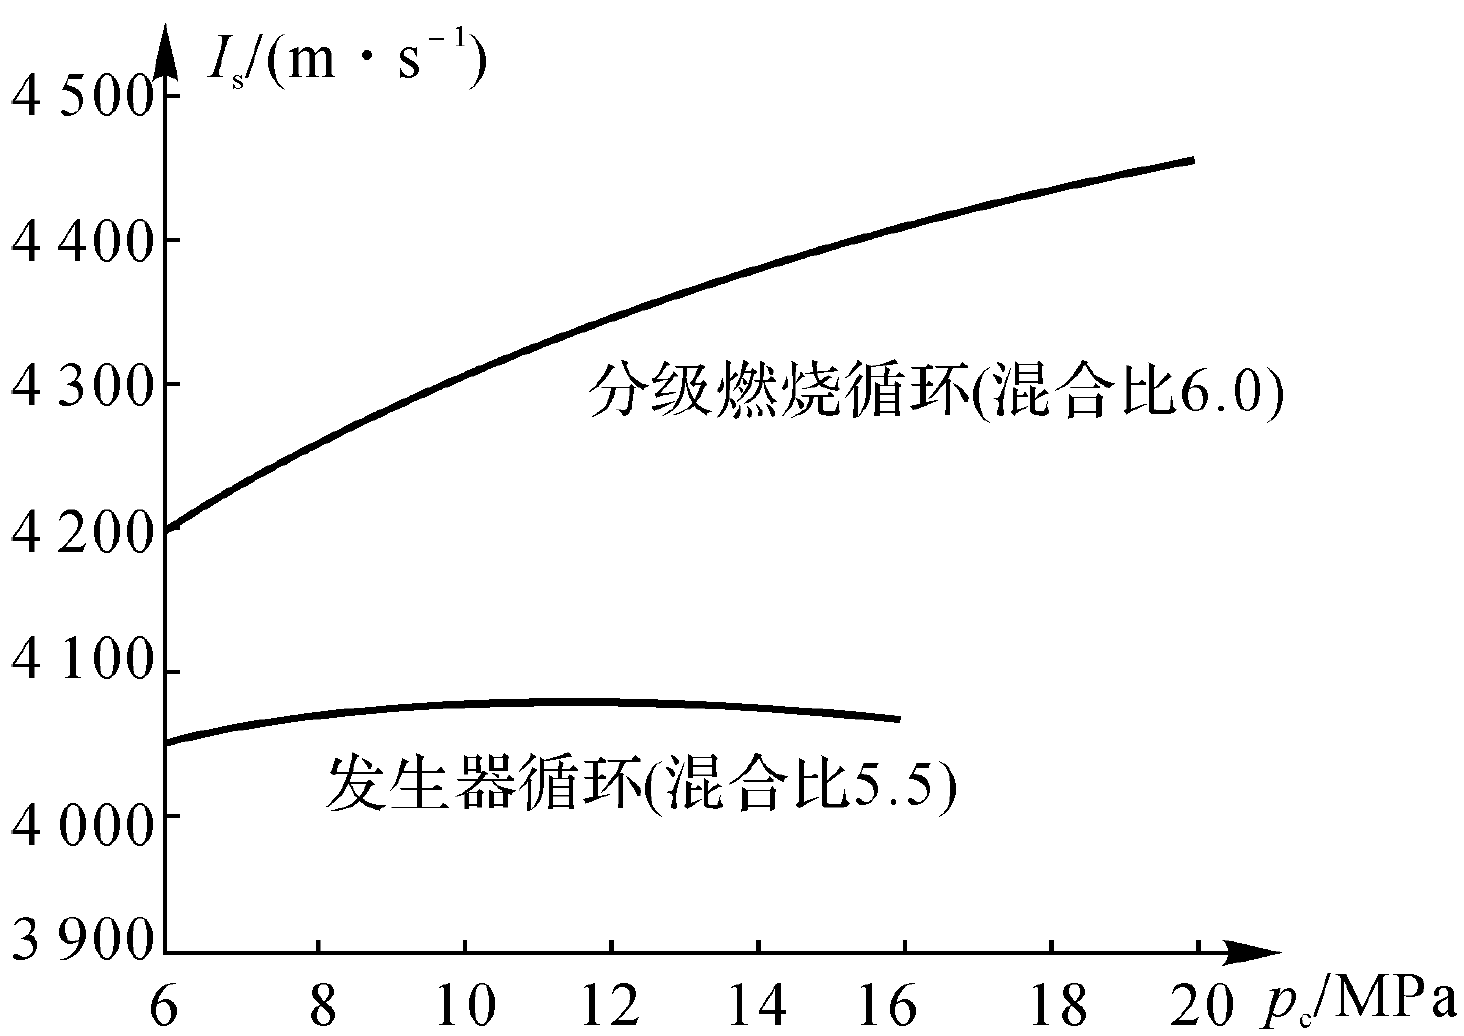
\includegraphics[width=0.935\linewidth]{pic/分级与燃气.png}
		\caption{分级燃烧循环和燃气发生器循环性能比较}
	\end{minipage}
\end{figure}


\subsection{推进剂贮箱增压系统}

\sssection[推进剂贮箱增压系统功能及分类]

\blue[功能]:保证贮箱内压强维持在一定的水平,确保发动机工作可靠。
\par 挤压式供应系统:与推进剂供应系统是一体的;
\par 泵压式供应系统:使推进剂贮箱保持一定的压强,以保证推进剂泵入口处的压强和流量满足要求 。

\blue[分类]
\begin{equation*}
	\begin{cases}
		\, \mbox{\makecell[c]{\dy[冷气增压系统]{LQZYXT} \newline (氮气、氦气)}}\,\, \longrightarrow \mbox{\makecell[c]{\dy[气瓶贮气增压系统]{QPZQZYXT}\newline(火箭总体提供)}}\\[0.5em]
		\, \mbox{\makecell[c]{\dy[热气增压系统]{RQZYXT}\newline (燃气)}}\,
		\begin{cases}
			\, \mbox{\dy[推进剂汽化增压系统]{TJJQHZYXT}}\\
			\, \mbox{\dy[燃气降温增压系统]{RQJWZYXT}}
		\end{cases}
	\end{cases}
\end{equation*}
\vspace*{0.5em}

\sssection[气瓶贮气增压系统]

\defination[气瓶贮气增压系统]
{
	\blue[原理]:利用高压气瓶中的冷态增压气体为贮箱中的推进剂增压。\\
	\hspace*{2em} \blue[基本组成]:气瓶、减压器、电磁阀或电爆阀,以及手动阀、单向阀、加温器等。\\
	\hspace*{2em} \blue[工质]:冷态增压气体常采用氮气和氦气,有沸点低、与推进剂及贮箱材料相容性好,摩尔质量不大的特点。\\
	\hspace*{2em} \blue[工作过程]:气瓶压强一般为$20\,$MPa$\, \sim \,35\,$MPa ,主电动气阀门打开,增压气体经减压器减压后,压强降为$3.5\, \sim \, 5.5\,$MPa ,然后分成两路分别进入推进剂贮箱,增压气体的流量由节流圈限定。
}

\warn[
\textbf{\large 气瓶贮气增压系统与冷气挤压式供应系统的区别和联系}\\
\hspace*{1.5em} (1) \hspace*{0.5em} \textbf{工作原理相同}:都是利用高压气瓶中的冷态增压气体进行增压。\\
\hspace*{1.5em} (2) \hspace*{0.5em} \textbf{使用目的不一样}:气瓶贮气增压系统是为贮箱中的推进剂增压,而冷气挤压式供应系统将液体推进剂挤压出来输送到推力室。\\
\hspace*{1.5em} (3) \hspace*{0.5em} \textbf{一般工作压强不一样}:气瓶贮气增压系统的工作压强一般为$20\,$MPa$\, \sim \,35\,$MPa ,冷气挤压式供应系统的工作压强一般低于气瓶气体压强20$\, \sim \,$35 MPa。
]
\vspace*{0.5em}

\sssection[推进剂汽化增压系统]

\defination[推进剂汽化增压系统]
{
	\blue[原理]:利用火箭自身携带的液体推进剂,经换热器汽化后来增压相应推进剂贮箱的一种增压系统(俗称自身增压系统)。\\
	\hspace*{2em} \blue[基本组成]:由音速喷嘴、蒸发器、单向阀、集合器、膜片阀及导管组成。\\
	\hspace*{2em} \blue[应用对象]:适用于热稳定性好、低沸点的推进剂(如\red[四氧化二氮]),特别是低分子量的低温推进剂(如液氢、液氧等)。\\
	\hspace*{2em} \blue[工作过程]:管内流推进剂,管外流涡轮废气,通过管长度和布置层次调节温度。
}

\sssection[燃气降温增压系统]

\defination[燃气降温增压系统]
{
	\blue[原理]:利用推进剂生成的燃气来增压相应推进剂贮箱,燃气一般取自为涡轮驱动提供工质的燃气发生器。\\
	\hspace*{2em} \blue[基本组成]:由音速喷嘴、燃气降温器、单向阀、集合器、膜片阀及导管组成。\\
	\hspace*{2em} \blue[工作过程]:从燃气发生器出口引出的一小股\red[富燃燃气] ,在\red[燃气降温器]中被燃料冷却后引出,再进入\red[增压燃料]贮箱 。氧化剂增压类似。管内流燃气,管外流冷却液,旁通路用来调节燃气温度。
}


\subsection{推进剂利用系统及其他分系统}

\sssection[1. 推进剂利用系统]

\underline{(1) \hspace*{0.3em} 推进剂利用系统原理}
\vspace*{0.5em}

用以保证推进剂组元同时耗尽、能自动进行推进剂组元混合比调节的系统。
\vspace*{-0.5em}

\warn
[
	\textbf{\large 为什么要需要推进剂利用系统?}\\
	\hspace*{2em} 在飞行过程中受各种因素(发动机性能、飞行器结构质量、飞行过载、气动加热及发动机制造造成的质量偏差)的影响,使实际混合比和加f注混合比与设计值有偏差,造成剩余,降低飞行器的运载能力。
]

\blue[工作原理]\quad 通过对供应系统中各组元流量的测量、反馈和对比分析,自动改变混合比,以减小或消除实际混合比和加注混合比的偏差,使所携带的推进剂全部消耗,或使剩余量最少,从而提高飞行器的运载能力。
\vspace*{0.5em}

\underline{(2) \hspace*{0.3em} 系统组成及部件功能}
\vspace*{0.5em}

\blue[基本组成]\quad 由液位传感器、变换器、利用系统控制机、放大器、推进剂调节阀门、电池、电缆等组成。
\begin{figure}[!htb]
	\centering
	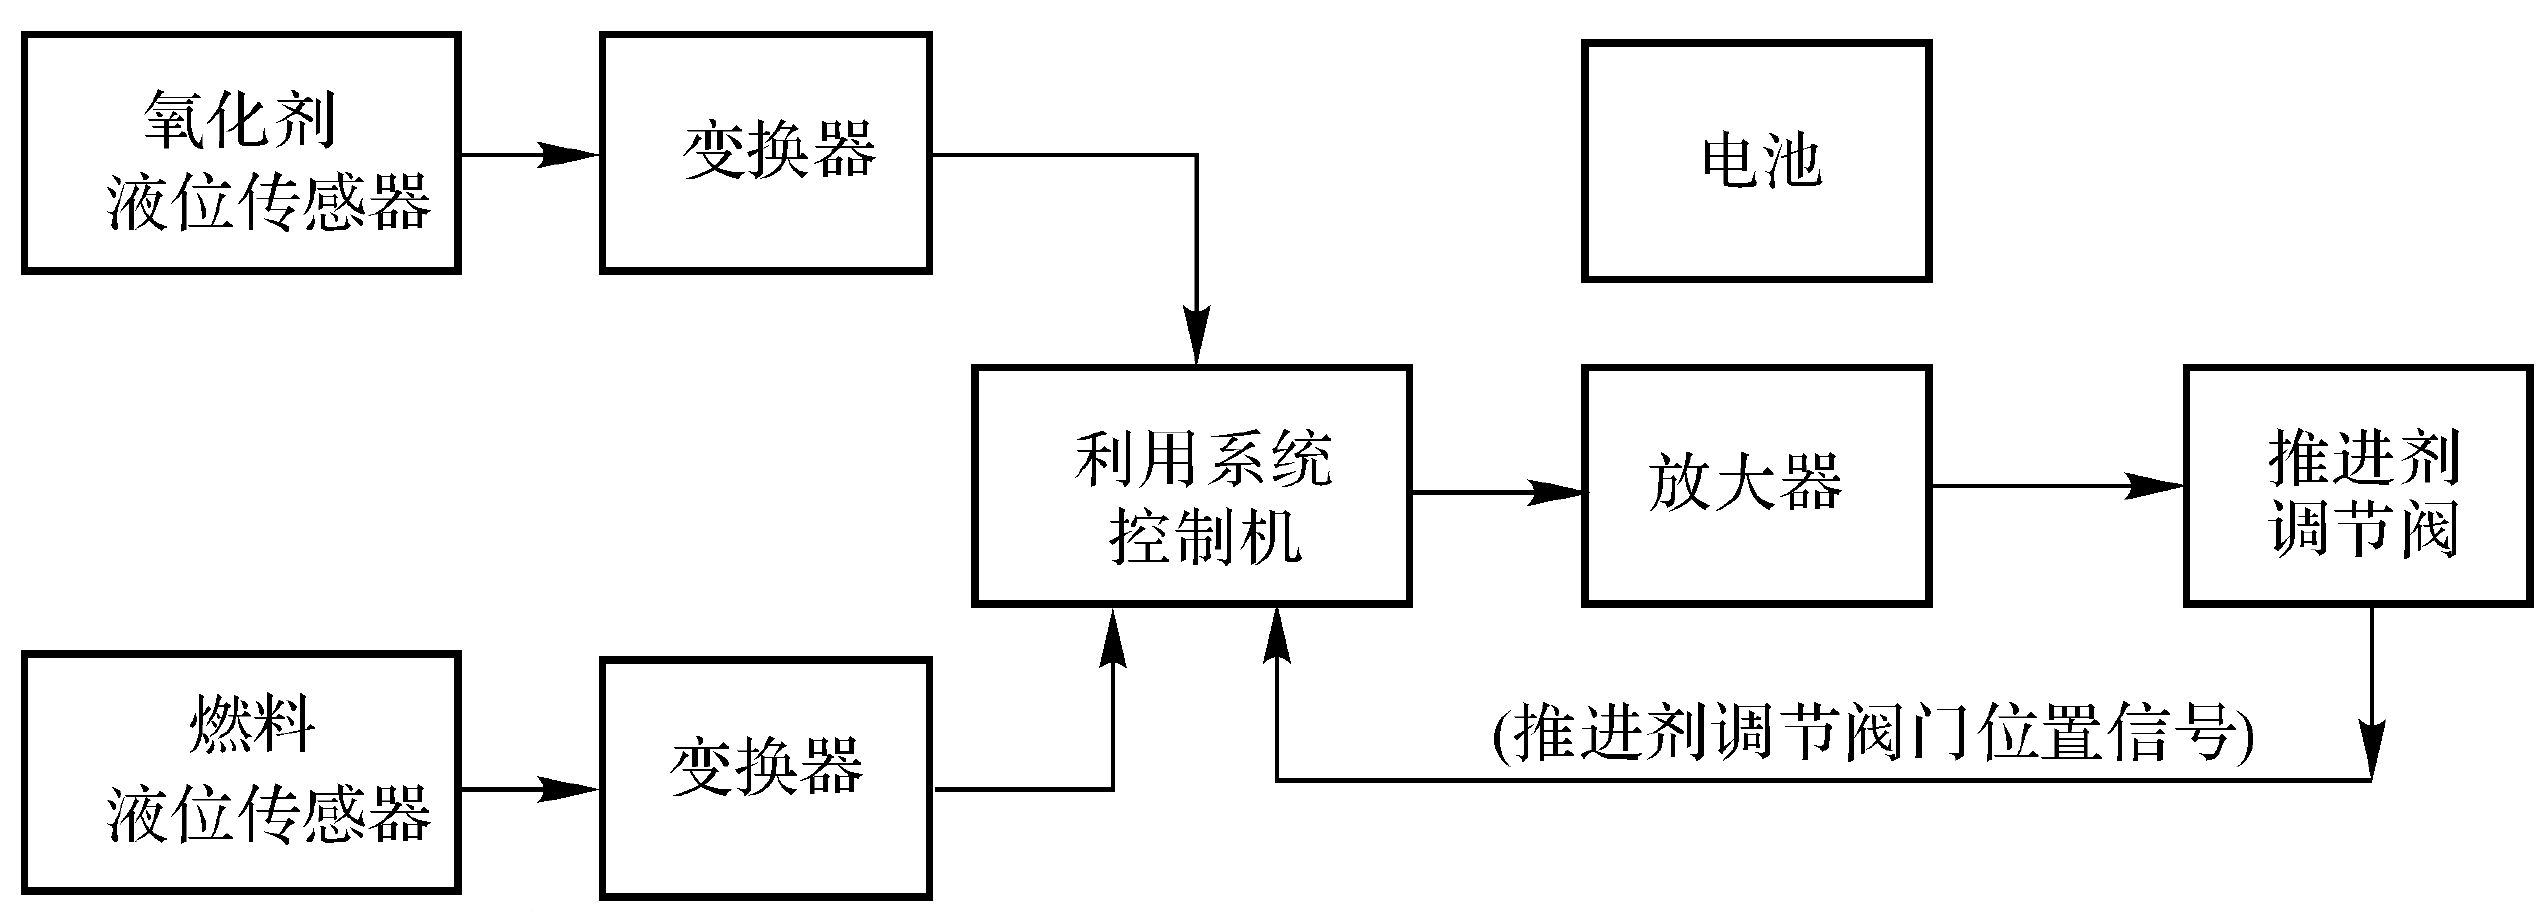
\includegraphics[width=0.7\linewidth]{pic/推进剂利用.png}
	\caption{推进剂利用系统组成}
\end{figure}

\blue[液位传感器]\quad 用来指示贮箱内推进剂液面高度的装置,有干簧式、电容式、电解式、浮子式、超声波式。

\blue[控制机]\quad 中枢,一台微型计算机,通常由单片机、接口及电路组成。功能:检测与处理液位信号;检测箭上控制系统输入的飞行时序指令(起飞、级间分离等);通过对控制方程计算,输出调节阀门的控制信号;识别遥测请求,输出利用系统的遥测信号等。

\blue[推进剂调节阀]\quad 是推进剂混合比调节的执行组件。
\vspace*{-0.5em}
\begin{enumerate}[\hspace*{3em}]
	\item \blue[工作原理]\quad 控制一种推进剂组元供应管路的流通横截面积,以改变推进剂流量、实现混合比调节。\vspace*{-0.5em}
	\item \blue[调节方式]
	\vspace*{-0.5em}
	\begin{itemize}
		\item 泵后回流: 将泵后一部分高压液体推进剂引回入泵前的低压区;\vspace*{-0.5em}
		\item 分流: 将泵后一部分高压推进剂不经过气蚀管直接进入推力室。\vspace*{-0.5em}
	\end{itemize}
	\item \blue[组成]
	\begin{equation*}
		\mbox{推进剂调节阀}
		\, \begin{cases}
			\, \mbox{阀门操作件} \,
			\begin{cases}
				\, \mbox{步进电机} \\
				\, \mbox{电动气阀}
			\end{cases}\\[1em]
			\, \mbox{调节件} \,
			\begin{cases}
				\, \mbox{比例调节阀:由步进电机操纵,流量连续变化} \\
				\, \mbox{常量调节阀:由电动气阀操纵,最大或最小,阶跃变化}
			\end{cases}
		\end{cases}
	\end{equation*}
\end{enumerate}

\underline{(3) \hspace*{0.3em} 系统工作原理}
\vspace*{0.5em}

\blue[起飞前] \quad  完成\red[接口初始化]和\red[调节阀门归零位] ,自检并与地面保持通信。

\blue[起飞后] \quad 传送状态参数,以\red[分离信号为零点]进入工作状态。

\blue[飞行过程中] 
\vspace*{-0.5em}
\begin{enumerate}[\hspace*{3em} $\bigstar$]
	\item 不断地对传感器进行检测;\vspace*{-0.5em}
	\item 根据预先装订的控制方程和数据进行计算;\vspace*{-0.5em}
	\item 发出修正控制信号,调节混合比;\vspace*{-0.5em}
	\item 同时将各种参数传给遥测系统。\vspace*{-0.5em}
\end{enumerate}

\vspace*{1em}

\sssection[吹除、置换和气封系统]

\underline{(1) \hspace*{0.3em} 吹除系统}
\vspace*{0.5em}

\blue[概念] \quad 用惰性气体将管道或腔体中的推进剂或气体吹掉。

\blue[分类] \quad 根据气源种类分为氮气和氦气吹除;根据气源压力分为强吹和弱吹。

\blue[作用]
\vspace*{-0.5em}
\begin{enumerate}[\hspace*{3em} $\bigstar$]
	\item 运载火箭的上面级,若需多次启动,关机后必须吹除,使发动机迅速关机,以减小后效冲量及其偏差、同时防止结冰堵塞管路与腔道。\vspace*{-0.5em}
	\item 液氧煤油发动机应有吹除系统,防止湿气凝结、燃气串腔,提高喷嘴压降,迅速关机,避免结焦。\vspace*{-0.5em}
	\item 氢氧发动机,加注前必须进行严格的系统吹除,防止爆炸,防止冻结导致的器件失灵、孔道堵塞等;还需舱段内吹除,防止空气液化。\vspace*{-0.5em}
\end{enumerate}
\vspace*{0.5em}

\underline{(2) \hspace*{0.3em} 置换系统}
\vspace*{0.5em}

\blue[功能] \quad 将推进剂贮箱和发动机系统腔道内的空气置换掉,使之达到技术条件的要求。
\blue[置换及要求] \quad 对于氢氧发动机,在液氢、液氧加注前必须对推进剂贮箱和发动机系统用\red[氦气进行严格的系统置换] ,目的是将贮箱氮气置换掉,使贮箱中的水蒸气、氧气、氮气含量符合技术要求。(水蒸气按露点控制,氧气小于30$\text{cm}^3$/$\text{m}^3$ ,氮气小于$\text{cm}^3$/$\text{m}^3$。

\blue[置换气体] \quad 一般是氢贮箱用氦气置换,氧贮箱用气态氧置换。
\vspace*{0.5em}

\underline{(3) \hspace*{0.3em} 气封系统}
\vspace*{0.5em}

\blue[低温抽吸效应] \quad 对于氢氧发动机,在液氢液氧加注过程中,会导致温度下降而抽吸周围空气,空气中的水蒸气结冰,将阀门冻死。

\blue[气封的作用] \quad 对排气口进行\red[正气压]保护,防止\dy[低温抽吸作用]{DWCXZY},防止阀门冻死。

\blue[气封的部位] \quad 氢氧排气管、氢氧贮箱增压管、氢氧溢流阀门控制管等。

\blue[组成] \quad 单向阀、限流嘴、导管等

\clearpage

\sssection[预冷系统]

\blue[作用] \quad 针对低温推进剂发动机,将管路、阀门和腔道等组件的温度降到液氢、液氧的温度,以防止低温推进剂流入时受热而汽化;避免两相流引起\red[泵失速]、\red[流量]和\red[压强波动]等等不良后果。

\blue[预冷系统]
\vspace*{-0.5em}
\begin{enumerate}[\hspace*{3em} $\bigstar$]
	\item \dy[自流式预冷]{ZLSYL}(\dy[排放式预冷]{PFSYL})\quad 将低温推进剂以一定流量流经系统,一直到主副系统的主、副阀门之前,经泄出口排向大气。\vspace*{-0.5em}
	\begin{itemize}
		\item 优点:结构简单。\vspace*{-0.5em}
		\item 缺点:消耗一定的推进剂。
	\end{itemize}
	一般发射前先由地面测试发控系统进行预冷 。上面级也需要预冷。
	\item \dy[回流式预冷]{HLSYL}(\dy[循环预冷]{XHYL})\quad 在发动机入口与推进剂贮箱入口之间增设回流泵,预冷的推进剂再返回到贮箱。\vspace*{-0.5em}
	\begin{itemize}
		\item 优点:无推进剂的消耗。
	\end{itemize}
	\vspace*{-0.5em}
\end{enumerate}
\vspace*{0.5em}

\subsection{涡轮泵与气蚀问题}

\sssection[涡轮泵功能及组成]

\defination[涡轮泵]
{
	\index{WLB@涡轮泵} 泵压式液体火箭发动机中涡轮和泵组合的总称,是液体火箭发动机的重要组成部分(\red[心脏]) 。
}

\blue[功能] \quad 将从贮箱中 来低压 推进剂组元的压力提高,并按发动机系统所要求的参数把推进剂输送到主推力室中;同时将部分或全部推进剂组元输入到燃气发生器或预燃室中,燃烧后的高温、高压燃气作为推动
涡轮的工质。

\blue[重要性] \quad 贮箱压力低,可\red[大大减轻结构质量];发动机性能的不断提高,需要更高的室压;涡轮泵在发动机中的作用越来越重要。

\blue[组成] \quad 由推进剂泵、涡轮、轴承、密封、齿轮传动系统、传速测量装置及辅助动力传动部分等组成。推进剂泵包括氧化剂泵和和燃料泵,有时还有涡轮工质泵。

\blue[涡轮和泵的传动和配置方式] \quad 同轴式、齿轮传动式、双涡轮式。
\vspace*{0.2em}

\blue[对涡轮泵的要求] 
\vspace*{-0.5em}
\begin{enumerate}[\hspace*{3em} $\bigstar$]
	\item 在给定的推进剂流量下,应保证发动机系统要求的\red[出口压力值];\vspace*{-0.5em}
	\item 具有最小的尺寸和结构质量;\vspace*{-0.5em}
	\item 具有尽可能\red[高的效率];\vspace*{-0.5em}
	\item 确保发动机在所有工况下稳定工作, \red[压力脉动与机械振动很小];\vspace*{-0.5em}
	\item 具有与腐蚀性液体或低温液体工作的相容性,不允许\red[氧化剂泵零件间有摩擦](这会导致局部加温,甚至爆炸);\vspace*{-0.5em}
	\item 具有高的\red[抗气蚀性能];\vspace*{-0.5em}
	\item 具有\red[抽吸含少量气体或蒸汽的推进剂]的能力。\vspace*{-0.5em}
\end{enumerate}
\vspace*{1em}

\sssection[涡轮泵的工作过程及特点]

其工作过程如图\ref{涡轮泵}所示。

\begin{figure}[!htb]
	\centering
	\begin{tikzpicture}
		\node (A) [draw, inner sep = 3pt]{\makecell[c]{$\,$燃气发生器$\,$\\[-0.5em]或预燃器}};
		\node (B) [draw, inner sep = 5pt, right of = A, node distance = 4.3cm]{涡轮喷嘴};
		\node (C) [draw, inner sep = 5pt, right of = B, node distance = 3.8cm]{涡轮动叶};
		\node (D) [draw, inner sep = 5pt, right of = C, node distance = 4.2cm]{涡轮转子};
		\node (E) [draw, below of = D ,inner sep = 5pt, node distance = 2cm]{齿轮或涡轮轴};
		\node (F) [draw, inner sep = 5pt, below of = C, node distance = 2cm, xshift = 0.6cm]{泵叶轮};
		\node (G) [draw, inner sep = 5pt, below of = B, node distance = 2cm, xshift = 0.6cm]{扩散器};
		\node (H) [draw, inner sep = 5pt, below of = A, node distance = 2cm]{推力室};
		
		\draw[-Stealth] (A) -- (B)node[midway, above = 0cm]{\small 燃气};
		\draw[-Stealth] (B) -- (C)node[midway, above = 0cm]{\small 热能$\rightarrow$动能};
		\draw[-Stealth] (C) -- (D)node[midway, above = 0cm]{\small 动能$\rightarrow$机械能};
		\draw[-Stealth] (D) -- (E) node[midway, left = 0cm]{\small 机械能传递};
		\draw[-Stealth] (E) -- (F);
		\draw[-Stealth] (F) -- (G)node[midway, above = 0cm]{\small 旋转};
		\draw[-Stealth] (G) -- (H)node[midway, above = 0cm]{\footnotesize 速度能$+$压力能$\leftarrow$机械能};
	\end{tikzpicture}
	\caption{涡轮泵的工作过程}
	\label{涡轮泵}
\end{figure}

\newpage 
\blue[主要特点]
\vspace*{-0.5em}
\begin{enumerate}[\hspace*{3em} $\bigstar$]
	\item \red[工作条件十分恶劣]。涡轮在高温、高压、高转速下工作;泵在常温、低温或超低温、高压、高转速的易燃、易爆、剧毒、强腐蚀的推进剂中工作。\vspace*{-0.5em}
	\item 涡轮泵结构复杂,零、部组件多,技术要求严,加工难度大,研究费用高,研制周期长,涡轮泵技术的综合性强,涉及技术领域广。\vspace*{-0.5em}
\end{enumerate}
\vspace*{1em}

\sssection[泵]

\underline{(1) \hspace*{0.3em} 泵的作用及分类}
\vspace*{0.3em}

\blue[作用] \quad 提高推进剂组元的压力,按一定的流量输送到推力室中去。

\blue[分类]\quad 容积式、引射式和叶片式, 液体火箭发动机 主要使用叶片式泵。
\vspace*{1em}

\underline{(2) \hspace*{0.3em} 叶片式泵}
\vspace*{0.5em}

安装在转轴的叶轮,流体经过高速旋转的叶轮后,其能量被提高。

\blue[优点] \quad 转速高、压头高、流量大、运动部件少、结构重量轻、外廓尺寸小,叶轮和壳体间隙大,不易造成摩擦生热,能够在\red[高、低温]以及\red[腐蚀介质]中工作;可以用电机和涡轮来传动。

\blue [缺点] \quad 当\red[进口压力小时,会发生汽蚀],从而影响正常工作;当流量变化时其压头会改变。
\vspace*{0.8em}

\blue[分类] \quad 
$
\begin{cases}
	\mbox{\dy[离心泵]{LXB}}\quad \mbox{作为主泵,广泛采用,主要介绍;}\\
	\mbox{\dy[轴流泵]{ZLB}}\quad \mbox{作为前置泵,称之为诱导泵,用来提高入口压力,提高抗气蚀的能力。}
\end{cases}
$
\vspace*{1em}

\underline{(3) \hspace*{0.3em} 离心泵的工作原理}
\vspace*{0.5em}

\dy[叶轮]{YL} \quad 高速旋转,在离心力作用下,液体推进剂被高速甩出叶轮 ,增加功能。

\dy[扩压器]{KYQ} \quad 从叶轮高速流出的推进剂进入扩压器,通道面积逐渐扩大,速度降低,动能逐渐下降而压力不断提升。

\blue[参数数量级]\quad 叶轮出口流体速度$50\, \sim \,100$ m / s;离心泵的出口流速$6\, \sim \,12$ m / s扬程:可贮存推进剂$300\, \sim \,500$ m ;低密度低温推进剂可达数万米 。

\vspace*{1em}

\underline{(4) \hspace*{0.3em} 泵的基本参数}
\vspace*{0.5em}

\dy[流量]{LL} \quad 单位时间内所抽送的液体体积或质量,分\dy[体积流量]{TJLL}和\dy[质量流量]{ZLLL}。

\dy[压头]{YT}(\dy[扬程]{YC})\quad 每一单位质量的液体通过泵后其\red[能量的增加值],H$\,$/$\,$m。

单位体积液体的能量为
\begin{equation}
	E = \rho gZ + p + \dfrac{1}{2}\rho v^2
\end{equation}
 两端同时除以$\rho$,可得
 \begin{equation}
 	\dfrac{E}{\rho} = gZ + \dfrac{p}{\rho} + \dfrac{v^2}{2} \quad (\text{J}\,/\,\text{kg})
 \end{equation}
 两端同时除以$g$,可得
 \begin{equation}
 	\dfrac{E}{\rho g} = Z + \dfrac{p}{\rho g} + \dfrac{v^2}{2 g} \quad (\text{m})
 \end{equation}
 单位质量液体流入和离开泵时的能量分别为
 \begin{align}
 	E_1 & = Z_1 + \dfrac{p_1}{\rho g} + \dfrac{v_1^2}{2g}\\
 	E_2 & = Z_2 + \dfrac{p_2}{\rho g} + \dfrac{v_2^2}{2g}
 \end{align}
所以泵给单位质量液体的能量为
\begin{equation}
	H = E_2 - E_1 = \dfrac{p_2 - p_1}{\rho g} + (Z_2 - Z_1) + \dfrac{v_2^2 - v_1^2}{2g}
\end{equation}
 其中,$p_1$为液体进入泵时的压力,$p_2$为液体流出泵时的压力;$v_1$为液体进入泵时的绝对速度,$v_2$为液体流出泵时的绝对速度;$Z_1$为泵进口液位高度,$Z_2$为泵出口液位高度;$g$为重力加速度。
 
\begin{figure}[!htb]
	\centering
	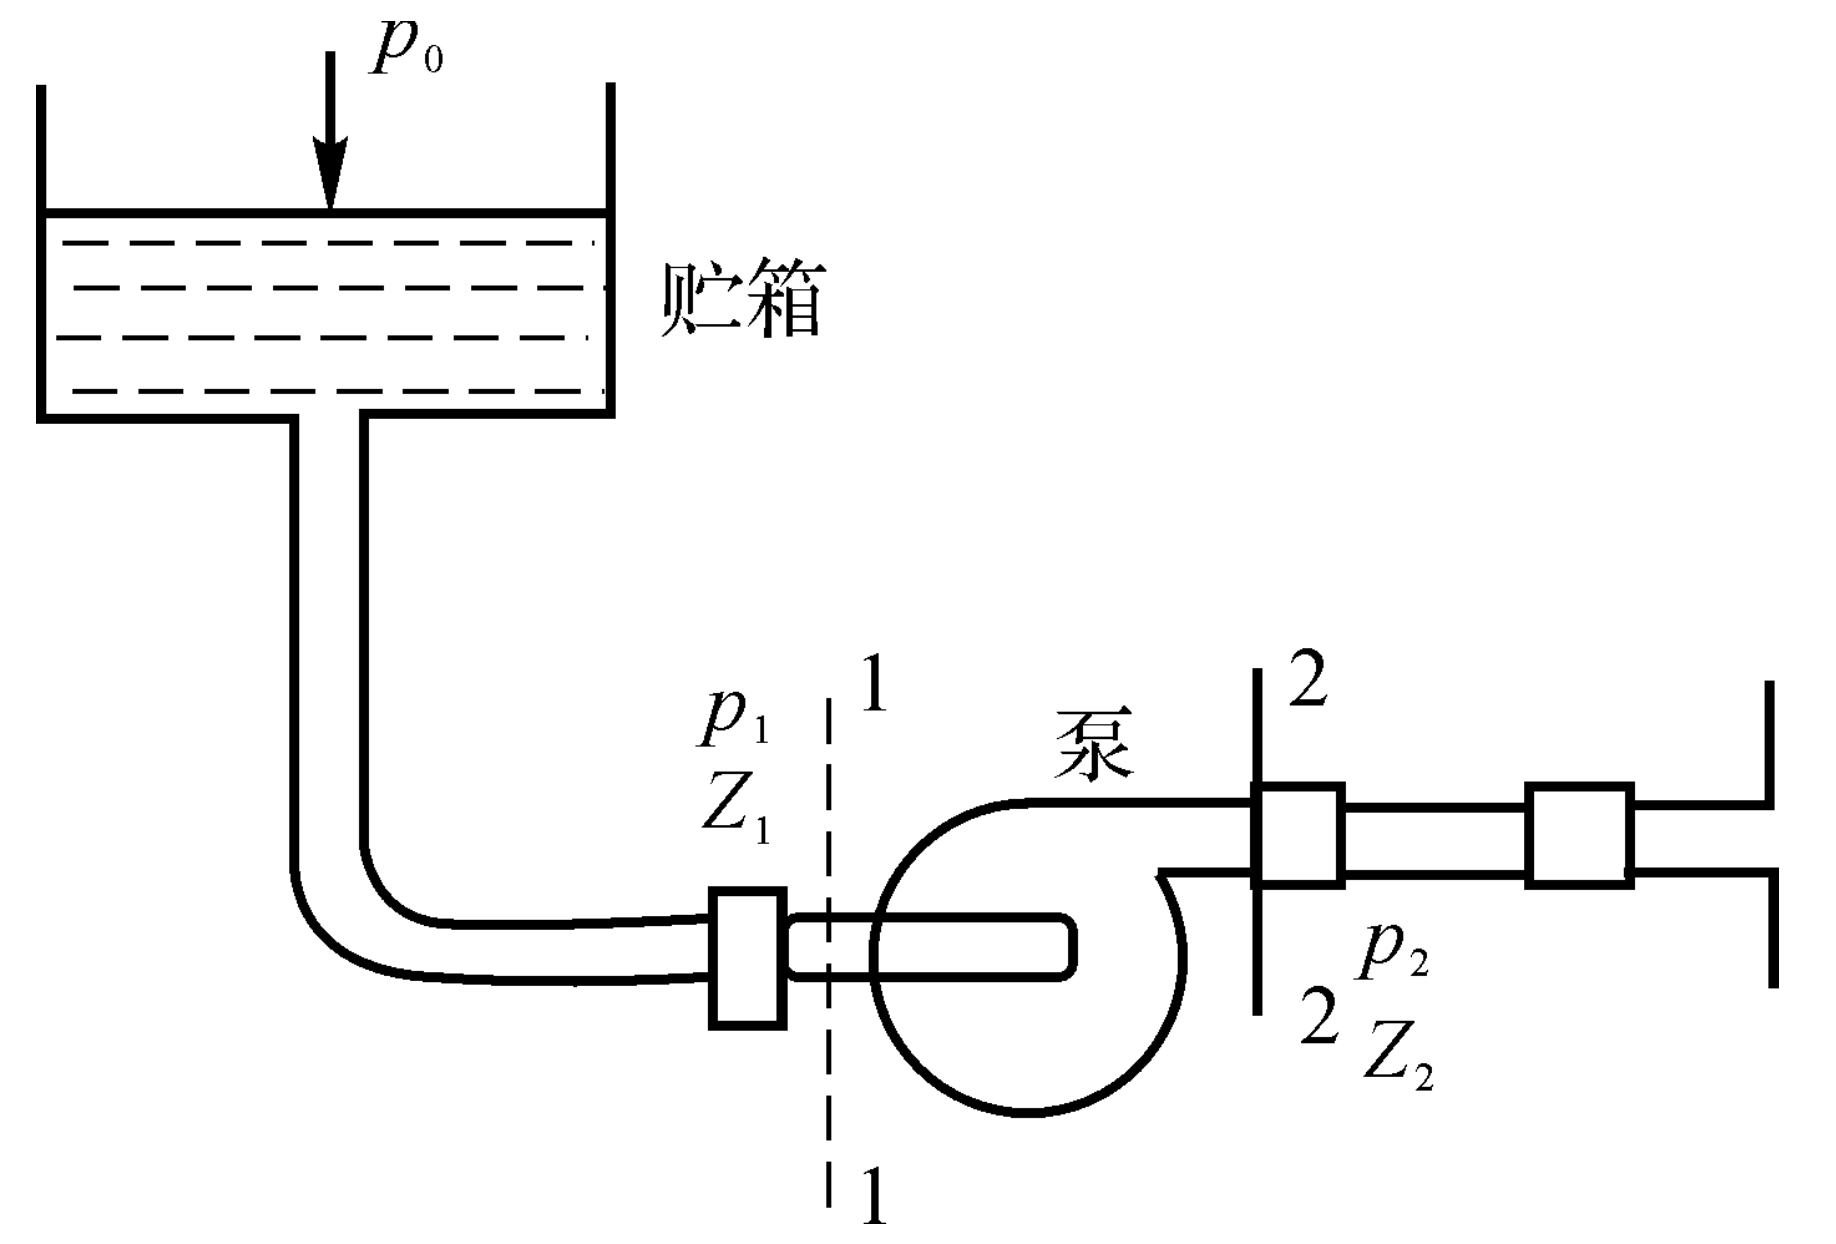
\includegraphics[width=0.4\linewidth]{pic/泵参数.png}
	\vspace*{-1em}
	\caption{泵的压头计算示意图}
\end{figure}

\dy[转速$n$]{ZS}\quad 在每分钟内转子的旋转圈数,r/min ,在设计时主要根据\red[泵的抗气蚀性能] 、结构布局、质量要求、轴承直径及密封切线速度等因素来确定。通常泵的转速为1000$\, \sim \,$4,000 r/min ,最高已达 9500 r/min 。

\dy[功率$P$]{GL}
\vspace*{-0.5em}
\begin{enumerate}[\hspace*{3em} $\bigstar$]
	\item \dy[输入功率]{SLGL} \quad 涡轮输送给泵的功率,或泵所消耗的功率。\vspace*{-0.5em}
	\item \dy[有效功率]{YXGL}\quad 在一定流量下,消耗在产生实际压头上的功率,或单位时间内流过泵的液体从泵那里所获得的能量。\vspace*{-0.5em}
\end{enumerate}

\dy[效率$\eta$]{XL} \quad 有效功率与输入功率之比$\eta_p$。

\vspace*{1em}


\underline{(5) \hspace*{0.3em} 泵的相似理论与比转速}

\defination[泵的相似理论与比转速]
{
	由于泵内液体运动的复杂性,需要广泛地应用模型试验来校核,为此要从\blue[实际粘性液体]的一般相似规律中,建立\blue[几何、运动、动力]的相似条件。根据\red[几何相似](形状和尺寸)和\red[运动相似](速度场)的条件建立相似泵间的主要关系。\red[利用速度三角形相似,得到实际泵和模型泵的比值]:
	\begin{equation}
		\dfrac{\bm{w}}{\bm{w}_\text{m}} = \dfrac{\bm{c}}{\bm{c}_\text{m}} = \dfrac{\bm{u}}{\bm{u}_\text{m}} = \text{Const} \qquad \dfrac{\bm{u}}{\bm{u}_\text{m}} = \dfrac{r \bm{n}}{r_\text{m}\bm{n}_\text{m}} = \lambda \dfrac{\bm{n}}{\bm{n}_\text{m}}
	\end{equation}	
	其中,$\bm{w}$为相对速度矢量,$\bm{c}$为绝对速度矢量,$\bm{u}$为圆周速度矢量,$\lambda$为尺寸比,下标m表示模型泵模型。
}

\clearpage

\noindent \textbf{\blue[【流量关系】]}

泵的体积流量为
\begin{equation}
	q_v = \pi D_2 b_2 k_2 c_{2\text{m}}\eta_v
\end{equation}
其中,$D_2$为泵叶轮外径,$b_2$为出口子午面的宽度,$k_2$为出口的排挤系数,$\eta_v$为泵的体积效率。

由几何相似,$k_2$相等,且有
\begin{equation}
	\dfrac{b_2}{b_{2\text{m}}} - \dfrac{D_2}{D_{2\text{m}}}, \qquad \dfrac{c_2}{c_{2 \text{m}}} = \dfrac{u_2}{u_{2 \text{m}}} = \dfrac{nD_2}{n_{\text{m}} D_{2 \text{m}}}
\end{equation}
略去$n_v$的差别,则有
\begin{equation}
	\dfrac{q_v}{q_{v\text{m}}} = \left(\dfrac{D_2}{D_{2 \text{m}}}\right)^3 \dfrac{n}{n_{\text{m}}}
\end{equation}
\vspace*{0.5em}

\noindent \textbf{\blue[【压头关系】]}
泵的压头可以写为
\begin{equation}
	H = (c_{2u}u_2 - c_{1u}u_1)\eta_h
\end{equation}
其中,$\eta_h$称为\dy[水力效率]{SLXL}。当实际泵与模型泵的尺寸和转速相差不大时,可以认为水力效率相等,再根据运动相似,其速度比为常数,则有
\begin{equation}
	\dfrac{H}{H_\text{m}} = \left(\dfrac{D_2}{D_{2\text{m}}}\right)^2 \left(\dfrac{n}{n_\text{m}}\right)^2
\end{equation}
\vspace*{0.5em}

\noindent \textbf{\blue[【功率关系】]} 
泵的输入功率可以写为$P_p = \dfrac{\rho q_V H}{\eta_p}$,认为泵效率相等,则有
\begin{equation}
	\dfrac{P_{\text{p}}}{P_{\text{pm}}} = \dfrac{\rho}{\rho_{\text{m}}} \left(\dfrac{D_2}{D_{2\text{m}}}\right)^5\left(\dfrac{n}{n_{\text{m}}}\right)^3
\end{equation}

\red[对于同一台泵,已知某一转速下的流量、压头和功率数据时,在转速变化不是很大的情况下,可以按等效率点换算出另一转速下的相应数据。]
\vspace*{0.5em}

\noindent \textbf{【\dy[比转速]{BZS}\blue[(综合性能参数)]】}

定义\dy[流量系数]{LLXS}
\begin{equation}
	\dfrac{q_{V}}{n D_2^3} = \dfrac{q_{V\text{m}}}{n_{\text{m}}D_{2\text{m}}^3} = \text{Const.}
	\label{流量系数}
\end{equation}
\dy[压头系数]{YTXS}
\begin{equation}
	\dfrac{H}{\big(n D_2\big)^2} = \dfrac{H_{\text{m}}}{\big(n_{\text{m}} D_{2\text{m}}\big)^2} = \text{Const.}
\end{equation}
\vspace*{0.5em}

将两个系数做适当处理,消去其中的尺寸参数,可得\dy[比转速]{BZS}
\begin{equation}
	\dfrac{\sqrt{\dfrac{q_V}{nD_2^3}}}{\left[\dfrac{H}{\big(n D_2\big)^2}\right]^{\textstyle \frac{3}{4}}} = \dfrac{n\sqrt{q_V}}{H^{\textstyle \frac{3}{4}}}
\end{equation}
\begin{equation*}
	\begin{cases}
		\, \mbox{当压头的单位为}\text{J / kg}\mbox{时有}n_\text{s} = \dfrac{20.24 n\sqrt{q_V}}{H^{\textstyle \frac{3}{4}}}\quad \mbox{(工程制单位)}\\[1.5em]
		\, \mbox{当压头的单位为 m 时有}n_\text{s} = \dfrac{3.65 n\sqrt{q_V}}{H^{\textstyle \frac{3}{4}}} \quad \mbox{(国际制单位)}
	\end{cases}
	\qquad \mbox{(两者相差} g^{\frac{3}{4}}\mbox{)}
\end{equation*}
\clearpage

\vspace*{-3em}
\warn
[
	(1) \hspace*{0.3em}对于多级泵,$H$按单级计算;对于双面进口叶轮,按单面入口流量计算;\\
	(2) \hspace*{0.3em}$n_s$是对应于最高效率点的工况值,如$i$级泵第一级为双面进口叶轮,则
	$n_s = \dfrac{3.65n\sqrt{q_v/2}}{\big(H/i\big)^{\textstyle \frac{3}{4}}}$\\
	(3) \hspace*{0.3em}几何相似、工况相似,则比转速相等;比转速相等泵不一定相似\\
	(4) \hspace*{0.3em}比转速是一个确定泵类型并影响泵级数选择的基本准测数。可以按$n_{\text{s}}$对泵及其特性曲线的趋势进行分类,即比转速是有因次的。
]
\vspace*{1em}

\sssection[泵气蚀的产生]

\defination[泵的气蚀和水力冲击]
{
	\dy[泵的气蚀]{BDQQ}\quad 当泵内局部区域的\red[静压力小于当地温度下的液体饱和蒸汽压力时]该处的液体即产生蒸汽泡,气泡随着液流进入高压区时,重新凝结并出现水击现象的全过程。\\[0.5em]
	\hspace*{2.5em}\dy[水力冲击]{SLCJ}\quad 当气泡进入较高的压力区时,气泡凝结形成液体,体积发生突然收缩 ,此刻大量的液体就以极大的加速度向着由于气泡凝结所形成的空腔中迅速冲来,形成巨大的水力冲击,可达几个大气压,几万赫兹。
}

\blue[气蚀过程]

\begin{figure}[!htb]
	\centering
	\begin{tikzpicture}
		\node (A) [draw, inner sep = 5pt]{高速流动};
		\node (B) [draw, inner sep = 5pt, right of = A, node distance = 5.3cm]{蒸汽泡};
		\node (C) [draw, inner sep = 5pt, right of = B, node distance = 4.8cm]{高压力区};
		\node (D) [draw, below of = C ,inner sep = 5pt, node distance = 2cm]{凝结成液体};
		\node (E) [draw, inner sep = 5pt, below of = B, node distance = 2cm]{高速液体汇聚};
		\node (F) [draw, inner sep = 5pt, below of = A, node distance = 2cm]{水力冲击};
		
		\draw[-Stealth] (A) -- (B)node[midway, above = 0cm]{\small 压强低于蒸汽压,沸腾};
		\draw[-Stealth] (B) -- (C)node[midway, above = 0cm]{\small 进入};
		\draw[-Stealth] (C) -- (D)node[midway, right = 0cm]{\small 压力改变};
		\draw[-Stealth] (D) -- (E)node[midway, above = 0cm]{\small 体积收缩};
		\draw[-Stealth] (E) -- (F)node[midway, above = 0cm]{\small 形成冲击力};
	\end{tikzpicture}
	\caption{泵的气蚀过程}
	\label{气蚀}
\end{figure}

\sssection[泵气蚀特征及改进措施]

\blue[(1)\hspace*{0.3em} 泵在发生气蚀时的特征]
\vspace*{-0.5em}
\begin{enumerate}[\hspace*{3em} $\bigstar$]
	\item \textbf{泵的流量、压头和效率,剧烈降低}: 泵发生气蚀后,叶轮通道被气蚀所阻塞,通道面积减小 $\rightarrow$ 流量降低;传递给叶轮的能量消耗在水力冲击上 压头、效率大大下降。\vspace*{-0.5em}
	\item \textbf{由于气蚀,泵会发生振动和噪音}。\vspace*{-0.5em}
	\item \textbf{泵的叶轮会发生机械损坏}: 很高的水利冲击会使金属剥落;分离出的氧原子会引起腐蚀。
\end{enumerate}

\blue[(2)\hspace*{0.3em} 提高抗气蚀的必要性及措施]
\vspace*{-0.5em}
\begin{enumerate}[\hspace*{3em} $\bigstar$]
	\item 由于气蚀具有上述危害,在液体发动机上泵是不允许发生气蚀;\vspace*{-0.5em}
	\item 为了提高涡轮的性能,减小尺寸和质量,尽可能提高涡轮泵的转速;而提高涡轮泵的性能受到抗气蚀的限制,因此必须设法提高泵抗气蚀的能力;\vspace*{-0.5em}
	\item 提高泵抗气蚀能力有多种方法,最有效发办法是采用组合泵,在离心泵前增加一个诱导轮,使离心轮进口液体压力提高,并使液体具有周向分速。
\end{enumerate}
\vspace*{0.5em}

\sssection[净正抽吸压头及气蚀比转速]

\blue[(1)\hspace*{0.3em} 不发生气蚀的条件]

在泵的入口处应具有一定的压力,使液体在泵内的流动过程中各处的静压不小于在该处温度下液体的饱和蒸汽压。
\vspace*{0.5em}

\blue[(2)\hspace*{0.3em} 泵入口压力的影响因素]

贮箱压力、液柱高度、惯性压力、进口管路的水力损失和动压头。
\vspace*{0.5em}

\blue[(3)]\hspace*{0.3em} \dy[净正抽吸压头]{JZCXYT}

在泵的入口处液体的总压头与在该处的温度下液体的饱和蒸气压头之差。泵的净正抽吸压力为
\begin{equation}
	H_{ne} = \dfrac{p_{ip}}{\rho g} + \dfrac{c_{ip}}{2g} - \dfrac{p_V}{\rho g}
\end{equation}
其中, $p_{ip}$为泵的入口压力;$p_V$为推进剂的饱和蒸汽压;$c_{ip}$为泵入口的轴向速度;$\rho$为推进剂的密度。
\vspace*{0.5em}

\blue[(4)]\hspace*{0.3em} \dy[净正抽吸压头临界值]{JZCXYTLJZ}

保证泵在一定的转速和流量下能正常工作的最低净正压头。通常取在额定工作状态下的泵压头下降不超过2\%$\sim$3\%最低净正抽吸压头。
\vspace*{0.5em}

\blue[(5)]\hspace*{0.3em} \dy[气蚀比转速]{QSBZS}

气蚀比转速是评价泵的抗气蚀性能的重要参数,由相似理论及公式\eqref{流量系数}可知
\begin{equation*}
	\dfrac{q_V}{D^3 n} = \text{Const.}
\end{equation*}
根据相似理论,可得
\begin{equation*}
	\dfrac{H_{ne}}{\big(Dn\big)^2} = \text{Const.}
\end{equation*}
将上面两个式子进行适当处理,消去尺寸参数$D$后,可得气蚀比转速
\begin{equation*}
	\begin{cases}
		\, \mbox{当压头的单位为}\text{J / kg}\mbox{时有}n_\text{ss} = \dfrac{31.2 n\sqrt{q_V}}{H^{\textstyle \frac{3}{4}}}\quad \mbox{(工程制单位)}\\[1.5em]
		\, \mbox{当压头的单位为 m 时有}n_\text{ss} = \dfrac{5.62 n\sqrt{q_V}}{H^{\textstyle \frac{3}{4}}} \quad \mbox{(国际制单位)}
	\end{cases}
	\qquad \mbox{(两者相差} g^{\frac{3}{4}}\mbox{)}
\end{equation*}

当泵是几何相似和运动相似时, $n_{\text{ss}}$为常数, $n_{\text{ss}}$可作为气蚀准则,表示气蚀性能的好坏; $n_{\text{ss}}$之值越大,泵的抗气蚀性能越好。
\vspace*{1em}

\sssection[诱导轮]\index{YDL@诱导轮}

\begin{figure}[!htb]
	\centering
	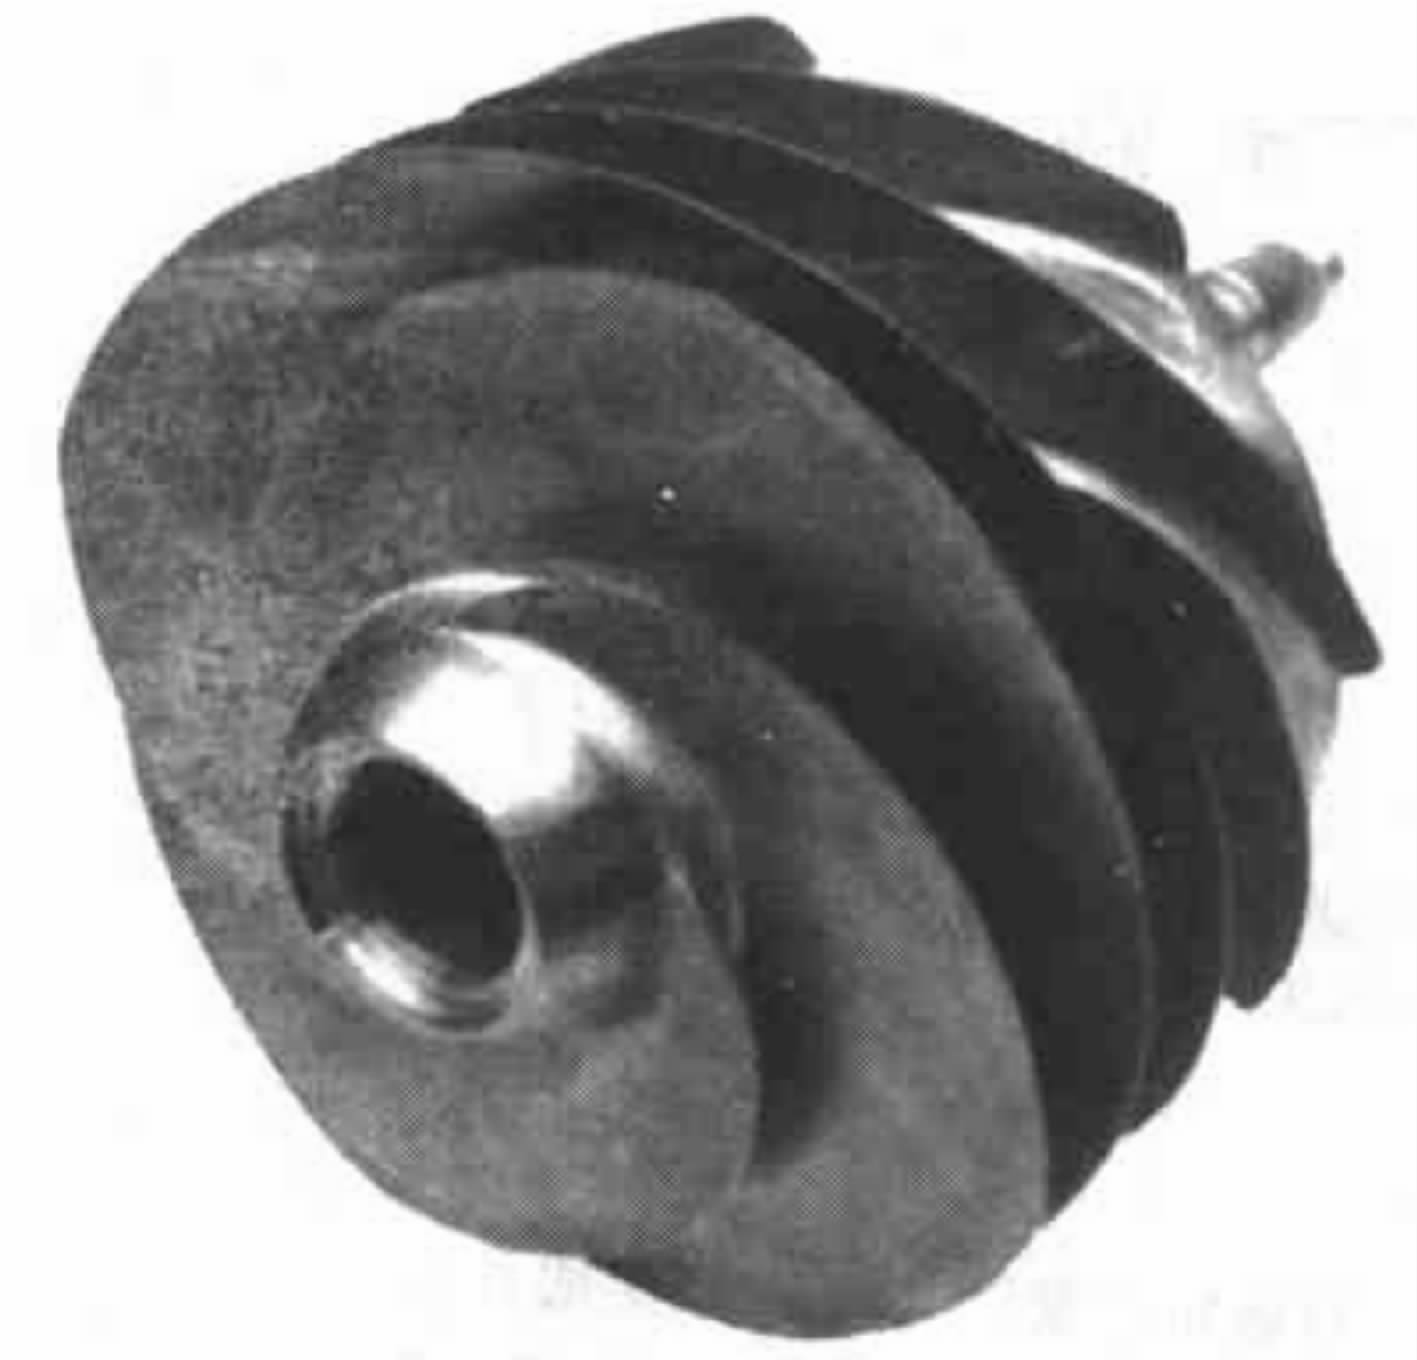
\includegraphics[width=0.25\linewidth]{pic/诱导轮.jpg}
	\caption{诱导轮}
\end{figure}

\blue[主要作用]\quad 用来提高主泵叶轮入口前的压力,以防止离心轮发生气蚀。

\blue[工作过程]\quad 如图 \ref{诱导轮} 所示。
\begin{figure}[!htb]
	\centering
	\begin{tikzpicture}
		\node (A) [draw = red, inner sep = 5pt, thick] {诱导轮};
		\node (B) [draw = blue, inner sep = 1pt, thick, right of = A,node distance = 3cm]{\makecell[c]{提高\\[-0.5em]$\,$涡轮泵转速$\,$}};
		\node (C) [draw = red, inner sep = 5pt, thick, right of = B, node distance = 3.8cm, yshift = 1cm]{减小尺寸和质量};
		\node (D) [draw = red, inner sep = 5pt, thick, right of = B, node distance = 3.8cm, yshift = 0cm]{提高抗气蚀性能};
		\node (E) [draw = red, inner sep = 5pt, thick, right of = B, node distance = 3.8cm, yshift = -1cm]{提高涡轮泵性能};
		\node (F) [draw = blue, inner sep = 1pt, thick, right of = D, node distance = 3.7cm]{\makecell[c]{降低\\[-0.5em]$\,$入口压力$\,$}};
		\node (G) [draw = red, inner sep = 1pt, thick, right of = F, node distance = 3.2cm, yshift = 0.8cm]{\makecell[c]{减小贮箱\\[-0.5em]$\,$结构质量$\,$}};
		\node (H) [draw = red, inner sep = 1pt, thick, right of = F, node distance = 3.2cm, yshift = -0.8cm]{\makecell[c]{减小增压\\[-0.5em]$\,$气体的量$\,$}};
		
		\draw [arrow] [draw = blue, thick] (A) -- (B);
		\draw [arrow] [draw = blue, thick] (B) --+(1.7cm, 0cm) --+ (1.7cm, 1cm) -- (C);
		\draw [arrow] [draw = blue, thick] (B) -- (D);
		\draw [arrow] [draw = blue, thick] (B) --+(1.7cm, 0cm) --+ (1.7cm, -1cm) -- (E);
		\draw [arrow] [draw = blue, thick] (D) -- (F);
		\draw [arrow] [draw = blue, thick] (F) --+(1.6cm, 0cm) --+ (1.6cm, 0.8cm) -- (G);
		\draw [arrow] [draw = blue, thick] (F) --+(1.6cm, 0cm) --+ (1.6cm, -0.8cm) -- (H);
	\end{tikzpicture}
	\caption{诱导轮的工作过程}
	\label{诱导轮}
\end{figure}

\blue[好处] \quad 采用诱导轮可使涡轮泵转速得以大幅度提高,不仅减小了涡轮泵的尺寸和质量,提高了涡轮泵的性能,而且由于抗气蚀性能提高,使泵可以在入口压力较低的情况下稳定可靠地工作,可减小贮箱的结构质量和增压气体的量。
\vspace*{1em}

\subsection{推力室组成及工作过程}

\sssection[推力室组成及特点]

\dy[推力室]{TLS}是发动机燃烧并产生推力的部件,是液体发动机的关键组件。
\begin{equation*}
	\mbox{推力室} \,
	\begin{cases}
		\, \mbox{头部} \,
			\begin{cases}
				\, \mbox{顶盖}\\
				\, \mbox{喷注器}\\
				\, \mbox{隔板:防止高频燃烧不稳定}
			\end{cases}
			\\[2.5em]
		\, \mbox{身部}
			\begin{cases}
				\, \mbox{圆柱段(燃烧室)}\\
				\, \mbox{喷管}
			\end{cases}
	\end{cases}
\end{equation*}

\blue[主要特点]
\vspace*{-0.5em}
\begin{enumerate}[\hspace*{3em} $\bigstar$]
	\item \red[燃烧室工作容积热容强度很大] ($10^3\sim10^4$MJ /($\text{m}^3$/s)), 比涡喷发动机大几十倍\vspace*{-0.5em}
	\item \red[燃烧室压强和温度均很高] (2$\sim$25 MPa, 4000 K 左右),对材料和冷却提出很苛刻的要求\vspace*{-0.5em}
	\item \red[燃烧组织有很大难度],单位截面推进剂流量很大,燃烧时间很短,燃烧效率要求很高\vspace*{-0.5em}
	\item \red[推进剂组元的每秒消耗量相当大] ,要求启动时能可靠地点燃推进剂。
\end{enumerate}
\vspace*{0.8em}

\sssection[推力室工作过程]

\blue[(1)\hspace*{0.3em} 推力室工作过程]

从向推力室内\red[喷入推进剂组元]开始,到\red[推进剂燃烧]转换为\red[燃烧产物] ,产物从\red[喷管喷出产生推力]为止的全部物理——化学过程。
\vspace*{0.5em}

\blue[(2)\hspace*{0.3em} 特点及要求]
\vspace*{-0.5em}
\begin{enumerate}[\hspace*{3em} $\bigstar$]
	\item 复杂的能量转换过程\vspace*{-0.5em}
	\item 在尺寸和重量都受限的推力室内,液体推进剂应迅速地燃烧或分解并放出热量\vspace*{-0.5em}
	\item 为得到最大的比推力,推进剂燃烧或分解时应放热最完全。
\end{enumerate}

\blue[(3)\hspace*{0.3em} 包含的基本物理化学方程]

推进剂的喷射雾化和液相混合过程、液滴的加热和蒸发过程、燃料和氧化剂的气相混合过程、混合气的燃烧化学反应过程等。

















